%
% sample root file for your "contribution" to a contributed volume
%
% Use this file as a template for your own input.
%
%%%%%%%%%%%%%%%% Springer %%%%%%%%%%%%%%%%%%%%%%%%%%%%%%%%%%
\documentclass[graybox,footinfo]{svmult}

\smartqed
\usepackage{mathptmx}       % selects Times Roman as basic font
\usepackage{helvet}         % selects Helvetica as sans-serif font
\usepackage{courier}        % selects Courier as typewriter font
\usepackage{type1cm}        % activate if the above 3 fonts are
% not available on your system
\usepackage{graphicx}       % standard LaTeX graphics tool
% when including figure files

\usepackage{array,colortbl}
\usepackage{amsmath,amsfonts,amssymb,bm} % no amsthm, Springer defines Theorem, Lemma, etc themselves
%\usepackage[mathx]{mathabx}
\DeclareFontFamily{U}{mathx}{\hyphenchar\font45}
\DeclareFontShape{U}{mathx}{m}{n}{
	<5> <6> <7> <8> <9> <10>
	<10.95> <12> <14.4> <17.28> <20.74> <24.88>
	mathx10
}{}
\DeclareSymbolFont{mathx}{U}{mathx}{m}{n}
\DeclareFontSubstitution{U}{mathx}{m}{n}
\DeclareMathAccent{\widecheck}      {0}{mathx}{"71}



% Note that Springer defines the following already:
%
% \D upright d for differential d
% \I upright i for imaginary unit
% \E upright e for exponential function
% \tens depicts tensors as sans serif upright
% \vec depicts vectors as boldface characters instead of the arrow accent
%
% Additionally we throw in the following common used macro's:
%%  This file will be included when we compile the final book. You can
%%  make use of the commonly used packages and commonly defined macros
%%  from here.
%%
%%  PLEASE DO NOT CHANGE THIS FILE.
%%  PLEASE DO NOT REDFINE ANY OF THE MACROS.
%%
%%  For convenience you may wish to define your own macros in your main
%%  tex file while preparing the manuscript. However, before submitting
%%  your final file for the accepted manuscript, we will ask you to replace
%%  your macros with the full commands.
%%

\renewcommand{\email}[1]{\emailname: #1} % change the email address font style

\usepackage{mathptmx}       % selects Times Roman as basic font
\usepackage{helvet}         % selects Helvetica as sans-serif font
\usepackage{courier}        % selects Courier as typewriter font
%\usepackage{type1cm}        % activate if the above 3 fonts are
%                            % not available on your system

\usepackage{makeidx}         % allows index generation
\usepackage{graphicx}        % standard LaTeX graphics tool
                             % when including figure files
%\usepackage{multicol}        % used for the two-column index
\usepackage[bottom]{footmisc}% places footnotes at page bottom

\usepackage{latexsym}
\usepackage{amsmath}
\usepackage{amsfonts}
\usepackage{amssymb}
\usepackage{bm}

\usepackage{url}
\usepackage{algorithm}
\usepackage{algorithmic}
\usepackage[misc,geometry]{ifsym}

% Springer provides the following environments:
%   case, conjecture, corollary, definition, example, exercise, lemma,
%   note, problem, property, proposition, question, remark, solution, theorem
%   claim, proof
\renewenvironment{proof}{\noindent{\itshape Proof.}}{\smartqed\qed}

% We add two more environments:   assumption, algo
\spdefaulttheorem{assumption}{Assumption}{\upshape \bfseries}{\itshape}
\spdefaulttheorem{algo}{Algorithm}{\upshape \bfseries}{\itshape}
% Note there is also the 'algorithm' environment from the algorithm package
% which is a floating environment



% Springer defines the following commands in math mode:
%   \D upright d for differential d
%   \I upright i for imaginary unit
%   \E upright e for exponential function
%   \tens depicts tensors as sans serif upright
%   \vec depicts vectors as boldface characters instead of the arrow accent


% We add the following commonly used macros:

% vectors as boldsymbols:
\newcommand{\bsa}{{\boldsymbol{a}}}
\newcommand{\bsb}{{\boldsymbol{b}}}
\newcommand{\bsc}{{\boldsymbol{c}}}
\newcommand{\bsd}{{\boldsymbol{d}}}
\newcommand{\bse}{{\boldsymbol{e}}}
\newcommand{\bsf}{{\boldsymbol{f}}}
\newcommand{\bsg}{{\boldsymbol{g}}}
\newcommand{\bsh}{{\boldsymbol{h}}}
\newcommand{\bsi}{{\boldsymbol{i}}}
\newcommand{\bsj}{{\boldsymbol{j}}}
\newcommand{\bsk}{{\boldsymbol{k}}}
\newcommand{\bsl}{{\boldsymbol{l}}}
\newcommand{\bsm}{{\boldsymbol{m}}}
\newcommand{\bsn}{{\boldsymbol{n}}}
\newcommand{\bso}{{\boldsymbol{o}}}
\newcommand{\bsp}{{\boldsymbol{p}}}
\newcommand{\bsq}{{\boldsymbol{q}}}
\newcommand{\bsr}{{\boldsymbol{r}}}
\newcommand{\bss}{{\boldsymbol{s}}}
\newcommand{\bst}{{\boldsymbol{t}}}
\newcommand{\bsu}{{\boldsymbol{u}}}
\newcommand{\bsv}{{\boldsymbol{v}}}
\newcommand{\bsw}{{\boldsymbol{w}}}
\newcommand{\bsx}{{\boldsymbol{x}}}
\newcommand{\bsy}{{\boldsymbol{y}}}
\newcommand{\bsz}{{\boldsymbol{z}}}
\newcommand{\bsA}{{\boldsymbol{A}}}
\newcommand{\bsB}{{\boldsymbol{B}}}
\newcommand{\bsC}{{\boldsymbol{C}}}
\newcommand{\bsD}{{\boldsymbol{D}}}
\newcommand{\bsE}{{\boldsymbol{E}}}
\newcommand{\bsF}{{\boldsymbol{F}}}
\newcommand{\bsG}{{\boldsymbol{G}}}
\newcommand{\bsH}{{\boldsymbol{H}}}
\newcommand{\bsI}{{\boldsymbol{I}}}
\newcommand{\bsJ}{{\boldsymbol{J}}}
\newcommand{\bsK}{{\boldsymbol{K}}}
\newcommand{\bsL}{{\boldsymbol{L}}}
\newcommand{\bsM}{{\boldsymbol{M}}}
\newcommand{\bsN}{{\boldsymbol{N}}}
\newcommand{\bsO}{{\boldsymbol{O}}}
\newcommand{\bsP}{{\boldsymbol{P}}}
\newcommand{\bsQ}{{\boldsymbol{Q}}}
\newcommand{\bsR}{{\boldsymbol{R}}}
\newcommand{\bsS}{{\boldsymbol{S}}}
\newcommand{\bsT}{{\boldsymbol{T}}}
\newcommand{\bsU}{{\boldsymbol{U}}}
\newcommand{\bsV}{{\boldsymbol{V}}}
\newcommand{\bsW}{{\boldsymbol{W}}}
\newcommand{\bsX}{{\boldsymbol{X}}}
\newcommand{\bsY}{{\boldsymbol{Y}}}
\newcommand{\bsZ}{{\boldsymbol{Z}}}
% other commonly used boldsymbols:
\newcommand{\bsell}{{\boldsymbol{\ell}}}
\newcommand{\bszero}{{\boldsymbol{0}}} % vector of zeros
\newcommand{\bsone}{{\boldsymbol{1}}}  % vector of ones
% boldsymbol greeks:
\newcommand{\bsalpha}{{\boldsymbol{\alpha}}}
\newcommand{\bsbeta}{{\boldsymbol{\beta}}}
\newcommand{\bsgamma}{{\boldsymbol{\gamma}}}
\newcommand{\bsdelta}{{\boldsymbol{\delta}}}
\newcommand{\bsepsilon}{{\boldsymbol{\epsilon}}}
\newcommand{\bsvarepsilon}{{\boldsymbol{\varepsilon}}}
\newcommand{\bszeta}{{\boldsymbol{\zeta}}}
\newcommand{\bseta}{{\boldsymbol{\eta}}}
\newcommand{\bstheta}{{\boldsymbol{\theta}}}
\newcommand{\bsvartheta}{{\boldsymbol{\vartheta}}}
\newcommand{\bskappa}{{\boldsymbol{\kappa}}}
\newcommand{\bslambda}{{\boldsymbol{\lambda}}}
\newcommand{\bsmu}{{\boldsymbol{\mu}}}
\newcommand{\bsnu}{{\boldsymbol{\nu}}}
\newcommand{\bsxi}{{\boldsymbol{\xi}}}
\newcommand{\bspi}{{\boldsymbol{\pi}}}
\newcommand{\bsvarpi}{{\boldsymbol{\varpi}}}
\newcommand{\bsrho}{{\boldsymbol{\rho}}}
\newcommand{\bsvarrho}{{\boldsymbol{\varrho}}}
\newcommand{\bssigma}{{\boldsymbol{\sigma}}}
\newcommand{\bsvarsigma}{{\boldsymbol{\varsigma}}}
\newcommand{\bstau}{{\boldsymbol{\tau}}}
\newcommand{\bsupsilon}{{\boldsymbol{\upsilon}}}
\newcommand{\bsphi}{{\boldsymbol{\phi}}}
\newcommand{\bsvarphi}{{\boldsymbol{\varphi}}}
\newcommand{\bschi}{{\boldsymbol{\chi}}}
\newcommand{\bspsi}{{\boldsymbol{\psi}}}
\newcommand{\bsomega}{{\boldsymbol{\omega}}}
\newcommand{\bsGamma}{{\boldsymbol{\Gamma}}}
\newcommand{\bsDelta}{{\boldsymbol{\Delta}}}
\newcommand{\bsTheta}{{\boldsymbol{\Theta}}}
\newcommand{\bsLambda}{{\boldsymbol{\Lambda}}}
\newcommand{\bsXi}{{\boldsymbol{\Xi}}}
\newcommand{\bsPi}{{\boldsymbol{\Pi}}}
\newcommand{\bsSigma}{{\boldsymbol{\Sigma}}}
\newcommand{\bsUpsilon}{{\boldsymbol{\Upsilon}}}
\newcommand{\bsPhi}{{\boldsymbol{\Phi}}}
\newcommand{\bsPsi}{{\boldsymbol{\Psi}}}
\newcommand{\bsOmega}{{\boldsymbol{\Omega}}}

% Roman fonts:
\newcommand{\rma}{{\mathrm{a}}}
\newcommand{\rmb}{{\mathrm{b}}}
\newcommand{\rmc}{{\mathrm{c}}}
\newcommand{\rmd}{{\mathrm{d}}}
\newcommand{\rme}{{\mathrm{e}}}
\newcommand{\rmf}{{\mathrm{f}}}
\newcommand{\rmg}{{\mathrm{g}}}
\newcommand{\rmh}{{\mathrm{h}}}
\newcommand{\rmi}{{\mathrm{i}}}
\newcommand{\rmj}{{\mathrm{j}}}
\newcommand{\rmk}{{\mathrm{k}}}
\newcommand{\rml}{{\mathrm{l}}}
\newcommand{\rmm}{{\mathrm{m}}}
\newcommand{\rmn}{{\mathrm{n}}}
\newcommand{\rmo}{{\mathrm{o}}}
\newcommand{\rmp}{{\mathrm{p}}}
\newcommand{\rmq}{{\mathrm{q}}}
\newcommand{\rmr}{{\mathrm{r}}}
\newcommand{\rms}{{\mathrm{s}}}
\newcommand{\rmt}{{\mathrm{t}}}
\newcommand{\rmu}{{\mathrm{u}}}
\newcommand{\rmv}{{\mathrm{v}}}
\newcommand{\rmw}{{\mathrm{w}}}
\newcommand{\rmx}{{\mathrm{x}}}
\newcommand{\rmy}{{\mathrm{y}}}
\newcommand{\rmz}{{\mathrm{z}}}
\newcommand{\rmA}{{\mathrm{A}}}
\newcommand{\rmB}{{\mathrm{B}}}
\newcommand{\rmC}{{\mathrm{C}}}
\newcommand{\rmD}{{\mathrm{D}}}
\newcommand{\rmE}{{\mathrm{E}}}
\newcommand{\rmF}{{\mathrm{F}}}
\newcommand{\rmG}{{\mathrm{G}}}
\newcommand{\rmH}{{\mathrm{H}}}
\newcommand{\rmI}{{\mathrm{I}}}
\newcommand{\rmJ}{{\mathrm{J}}}
\newcommand{\rmK}{{\mathrm{K}}}
\newcommand{\rmL}{{\mathrm{L}}}
\newcommand{\rmM}{{\mathrm{M}}}
\newcommand{\rmN}{{\mathrm{N}}}
\newcommand{\rmO}{{\mathrm{O}}}
\newcommand{\rmP}{{\mathrm{P}}}
\newcommand{\rmQ}{{\mathrm{Q}}}
\newcommand{\rmR}{{\mathrm{R}}}
\newcommand{\rmS}{{\mathrm{S}}}
\newcommand{\rmT}{{\mathrm{T}}}
\newcommand{\rmU}{{\mathrm{U}}}
\newcommand{\rmV}{{\mathrm{V}}}
\newcommand{\rmW}{{\mathrm{W}}}
\newcommand{\rmX}{{\mathrm{X}}}
\newcommand{\rmY}{{\mathrm{Y}}}
\newcommand{\rmZ}{{\mathrm{Z}}}
% also commonly defined
\newcommand{\rd}{{\mathrm{d}}}
\newcommand{\ri}{{\mathrm{i}}}

% blackboards:
\newcommand{\bbA}{{\mathbb{A}}}
\newcommand{\bbB}{{\mathbb{B}}}
\newcommand{\bbC}{{\mathbb{C}}}
\newcommand{\bbD}{{\mathbb{D}}}
\newcommand{\bbE}{{\mathbb{E}}}
\newcommand{\bbF}{{\mathbb{F}}}
\newcommand{\bbG}{{\mathbb{G}}}
\newcommand{\bbH}{{\mathbb{H}}}
\newcommand{\bbI}{{\mathbb{I}}}
\newcommand{\bbJ}{{\mathbb{J}}}
\newcommand{\bbK}{{\mathbb{K}}}
\newcommand{\bbL}{{\mathbb{L}}}
\newcommand{\bbM}{{\mathbb{M}}}
\newcommand{\bbN}{{\mathbb{N}}}
\newcommand{\bbO}{{\mathbb{O}}}
\newcommand{\bbP}{{\mathbb{P}}}
\newcommand{\bbQ}{{\mathbb{Q}}}
\newcommand{\bbR}{{\mathbb{R}}}
\newcommand{\bbS}{{\mathbb{S}}}
\newcommand{\bbT}{{\mathbb{T}}}
\newcommand{\bbU}{{\mathbb{U}}}
\newcommand{\bbV}{{\mathbb{V}}}
\newcommand{\bbW}{{\mathbb{W}}}
\newcommand{\bbX}{{\mathbb{X}}}
\newcommand{\bbY}{{\mathbb{Y}}}
\newcommand{\bbZ}{{\mathbb{Z}}}
% commonly used shortcuts:
\newcommand{\C}{{\mathbb{C}}} % complex numbers
\newcommand{\F}{{\mathbb{F}}} % field, finite field
\newcommand{\N}{{\mathbb{N}}} % natural numbers {1, 2, ...}
\newcommand{\Q}{{\mathbb{Q}}} % rationals
\newcommand{\R}{{\mathbb{R}}} % reals
\newcommand{\Z}{{\mathbb{Z}}} % integers
% more commonly used shortcuts:
\newcommand{\CC}{{\mathbb{C}}} % complex numbers
\newcommand{\FF}{{\mathbb{F}}} % field, finite field
\newcommand{\NN}{{\mathbb{N}}} % natural numbers {1, 2, ...}
\newcommand{\QQ}{{\mathbb{Q}}} % rationals
\newcommand{\RR}{{\mathbb{R}}} % reals
\newcommand{\ZZ}{{\mathbb{Z}}} % integers
% more commonly used shortcuts:
\newcommand{\EE}{{\mathbb{E}}}
\newcommand{\PP}{{\mathbb{P}}}
\newcommand{\TT}{{\mathbb{T}}}
\newcommand{\VV}{{\mathbb{V}}}
% and even more commonly used shortcuts:
\newcommand{\Complex}{{\mathbb{C}}}
\newcommand{\Integer}{{\mathbb{Z}}}
\newcommand{\Natural}{{\mathbb{N}}}
\newcommand{\Rational}{{\mathbb{Q}}}
\newcommand{\Real}{{\mathbb{R}}}
% indicator boldface 1:
\DeclareSymbolFont{bbold}{U}{bbold}{m}{n}
\DeclareSymbolFontAlphabet{\mathbbold}{bbold}
\newcommand{\ind}{{\mathbbold{1}}}
\newcommand{\bbone}{{\mathbbold{1}}}


% calligraphic letters:
\newcommand{\cala}{{\mathcal{a}}}
\newcommand{\calb}{{\mathcal{b}}}
\newcommand{\calc}{{\mathcal{c}}}
\newcommand{\cald}{{\mathcal{d}}}
\newcommand{\cale}{{\mathcal{e}}}
\newcommand{\calf}{{\mathcal{f}}}
\newcommand{\calg}{{\mathcal{g}}}
\newcommand{\calh}{{\mathcal{h}}}
\newcommand{\cali}{{\mathcal{i}}}
\newcommand{\calj}{{\mathcal{j}}}
\newcommand{\calk}{{\mathcal{k}}}
\newcommand{\call}{{\mathcal{l}}}
\newcommand{\calm}{{\mathcal{m}}}
\newcommand{\caln}{{\mathcal{n}}}
\newcommand{\calo}{{\mathcal{o}}}
\newcommand{\calp}{{\mathcal{p}}}
\newcommand{\calq}{{\mathcal{q}}}
\newcommand{\calr}{{\mathcal{r}}}
\newcommand{\cals}{{\mathcal{s}}}
\newcommand{\calt}{{\mathcal{t}}}
\newcommand{\calu}{{\mathcal{u}}}
\newcommand{\calv}{{\mathcal{v}}}
\newcommand{\calw}{{\mathcal{w}}}
\newcommand{\calx}{{\mathcal{x}}}
\newcommand{\caly}{{\mathcal{y}}}
\newcommand{\calz}{{\mathcal{z}}}
\newcommand{\calA}{{\mathcal{A}}}
\newcommand{\calB}{{\mathcal{B}}}
\newcommand{\calC}{{\mathcal{C}}}
\newcommand{\calD}{{\mathcal{D}}}
\newcommand{\calE}{{\mathcal{E}}}
\newcommand{\calF}{{\mathcal{F}}}
\newcommand{\calG}{{\mathcal{G}}}
\newcommand{\calH}{{\mathcal{H}}}
\newcommand{\calI}{{\mathcal{I}}}
\newcommand{\calJ}{{\mathcal{J}}}
\newcommand{\calK}{{\mathcal{K}}}
\newcommand{\calL}{{\mathcal{L}}}
\newcommand{\calM}{{\mathcal{M}}}
\newcommand{\calN}{{\mathcal{N}}}
\newcommand{\calO}{{\mathcal{O}}}
\newcommand{\calP}{{\mathcal{P}}}
\newcommand{\calQ}{{\mathcal{Q}}}
\newcommand{\calR}{{\mathcal{R}}}
\newcommand{\calS}{{\mathcal{S}}}
\newcommand{\calT}{{\mathcal{T}}}
\newcommand{\calU}{{\mathcal{U}}}
\newcommand{\calV}{{\mathcal{V}}}
\newcommand{\calW}{{\mathcal{W}}}
\newcommand{\calX}{{\mathcal{X}}}
\newcommand{\calY}{{\mathcal{Y}}}
\newcommand{\calZ}{{\mathcal{Z}}}

% Euler fraks:
\newcommand{\fraka}{{\mathfrak{a}}}
\newcommand{\frakb}{{\mathfrak{b}}}
\newcommand{\frakc}{{\mathfrak{c}}}
\newcommand{\frakd}{{\mathfrak{d}}}
\newcommand{\frake}{{\mathfrak{e}}}
\newcommand{\frakf}{{\mathfrak{f}}}
\newcommand{\frakg}{{\mathfrak{g}}}
\newcommand{\frakh}{{\mathfrak{h}}}
\newcommand{\fraki}{{\mathfrak{i}}}
\newcommand{\frakj}{{\mathfrak{j}}}
\newcommand{\frakk}{{\mathfrak{k}}}
\newcommand{\frakl}{{\mathfrak{l}}}
\newcommand{\frakm}{{\mathfrak{m}}}
\newcommand{\frakn}{{\mathfrak{n}}}
\newcommand{\frako}{{\mathfrak{o}}}
\newcommand{\frakp}{{\mathfrak{p}}}
\newcommand{\frakq}{{\mathfrak{q}}}
\newcommand{\frakr}{{\mathfrak{r}}}
\newcommand{\fraks}{{\mathfrak{s}}}
\newcommand{\frakt}{{\mathfrak{t}}}
\newcommand{\fraku}{{\mathfrak{u}}}
\newcommand{\frakv}{{\mathfrak{v}}}
\newcommand{\frakw}{{\mathfrak{w}}}
\newcommand{\frakx}{{\mathfrak{x}}}
\newcommand{\fraky}{{\mathfrak{y}}}
\newcommand{\frakz}{{\mathfrak{z}}}
\newcommand{\frakA}{{\mathfrak{A}}}
\newcommand{\frakB}{{\mathfrak{B}}}
\newcommand{\frakC}{{\mathfrak{C}}}
\newcommand{\frakD}{{\mathfrak{D}}}
\newcommand{\frakE}{{\mathfrak{E}}}
\newcommand{\frakF}{{\mathfrak{F}}}
\newcommand{\frakG}{{\mathfrak{G}}}
\newcommand{\frakH}{{\mathfrak{H}}}
\newcommand{\frakI}{{\mathfrak{I}}}
\newcommand{\frakJ}{{\mathfrak{J}}}
\newcommand{\frakK}{{\mathfrak{K}}}
\newcommand{\frakL}{{\mathfrak{L}}}
\newcommand{\frakM}{{\mathfrak{M}}}
\newcommand{\frakN}{{\mathfrak{N}}}
\newcommand{\frakO}{{\mathfrak{O}}}
\newcommand{\frakP}{{\mathfrak{P}}}
\newcommand{\frakQ}{{\mathfrak{Q}}}
\newcommand{\frakR}{{\mathfrak{R}}}
\newcommand{\frakS}{{\mathfrak{S}}}
\newcommand{\frakT}{{\mathfrak{T}}}
\newcommand{\frakU}{{\mathfrak{U}}}
\newcommand{\frakV}{{\mathfrak{V}}}
\newcommand{\frakW}{{\mathfrak{W}}}
\newcommand{\frakX}{{\mathfrak{X}}}
\newcommand{\frakY}{{\mathfrak{Y}}}
\newcommand{\frakZ}{{\mathfrak{Z}}}
% sets as Euler fraks:
\newcommand{\seta}{{\mathfrak{a}}}
\newcommand{\setb}{{\mathfrak{b}}}
\newcommand{\setc}{{\mathfrak{c}}}
\newcommand{\setd}{{\mathfrak{d}}}
\newcommand{\sete}{{\mathfrak{e}}}
\newcommand{\setf}{{\mathfrak{f}}}
\newcommand{\setg}{{\mathfrak{g}}}
\newcommand{\seth}{{\mathfrak{h}}}
\newcommand{\seti}{{\mathfrak{i}}}
\newcommand{\setj}{{\mathfrak{j}}}
\newcommand{\setk}{{\mathfrak{k}}}
\newcommand{\setl}{{\mathfrak{l}}}
\newcommand{\setm}{{\mathfrak{m}}}
\newcommand{\setn}{{\mathfrak{n}}}
\newcommand{\seto}{{\mathfrak{o}}}
\newcommand{\setp}{{\mathfrak{p}}}
\newcommand{\setq}{{\mathfrak{q}}}
\newcommand{\setr}{{\mathfrak{r}}}
\newcommand{\sets}{{\mathfrak{s}}}
\newcommand{\sett}{{\mathfrak{t}}}
\newcommand{\setu}{{\mathfrak{u}}}
\newcommand{\setv}{{\mathfrak{v}}}
\newcommand{\setw}{{\mathfrak{w}}}
\newcommand{\setx}{{\mathfrak{x}}}
\newcommand{\sety}{{\mathfrak{y}}}
\newcommand{\setz}{{\mathfrak{z}}}
\newcommand{\setA}{{\mathfrak{A}}}
\newcommand{\setB}{{\mathfrak{B}}}
\newcommand{\setC}{{\mathfrak{C}}}
\newcommand{\setD}{{\mathfrak{D}}}
\newcommand{\setE}{{\mathfrak{E}}}
\newcommand{\setF}{{\mathfrak{F}}}
\newcommand{\setG}{{\mathfrak{G}}}
\newcommand{\setH}{{\mathfrak{H}}}
\newcommand{\setI}{{\mathfrak{I}}}
\newcommand{\setJ}{{\mathfrak{J}}}
\newcommand{\setK}{{\mathfrak{K}}}
\newcommand{\setL}{{\mathfrak{L}}}
\newcommand{\setM}{{\mathfrak{M}}}
\newcommand{\setN}{{\mathfrak{N}}}
\newcommand{\setO}{{\mathfrak{O}}}
\newcommand{\setP}{{\mathfrak{P}}}
\newcommand{\setQ}{{\mathfrak{Q}}}
\newcommand{\setR}{{\mathfrak{R}}}
\newcommand{\setS}{{\mathfrak{S}}}
\newcommand{\setT}{{\mathfrak{T}}}
\newcommand{\setU}{{\mathfrak{U}}}
\newcommand{\setV}{{\mathfrak{V}}}
\newcommand{\setW}{{\mathfrak{W}}}
\newcommand{\setX}{{\mathfrak{X}}}
\newcommand{\setY}{{\mathfrak{Y}}}
\newcommand{\setZ}{{\mathfrak{Z}}}

% other commonly defined commands:
\newcommand{\wal}{{\rm wal}}
\newcommand{\floor}[1]{\left\lfloor #1 \right\rfloor} % floor
\newcommand{\ceil}[1]{\left\lceil #1 \right\rceil}    % ceil
\DeclareMathOperator{\cov}{Cov}
\DeclareMathOperator{\var}{Var}
\providecommand{\argmin}{\operatorname*{argmin}}
\providecommand{\argmax}{\operatorname*{argmax}}


% Macros below are now included in macros.tex from MCQMC 2016 web site
% This spot formerly included macros that are now in macros.tex

% indicator boldface 1:
\DeclareSymbolFont{bbold}{U}{bbold}{m}{n}
\DeclareSymbolFontAlphabet{\mathbbold}{bbold}
%\newcommand{\ind}{\mathbbold{1}}


\usepackage{microtype} % good font tricks

\usepackage[colorlinks=true,linkcolor=black,citecolor=black,urlcolor=black]{hyperref}
\urlstyle{same}
\usepackage{bookmark}
\pdfstringdefDisableCommands{\def\and{, }}
\makeatletter % to avoid hyperref warnings:
\providecommand*{\toclevel@author}{999}
\providecommand*{\toclevel@title}{0}
\makeatother



\usepackage{bbm,mathtools,array,longtable,booktabs,graphicx,color,enumitem}
%\input FJHDef.tex


\newcommand{\QMCPYnorm}[2][{}]{\ensuremath{\left \lVert #2 \right \rVert}_{#1}}
\newcommand{\QMCPYnormnorm}[2][{}]{\ensuremath{\lVert #2 \rVert}_{#1}}
\newcommand{\QMCPYbignorm}[2][{}]{\ensuremath{\bigl \lVert #2 \bigr \rVert}_{#1}}
\newcommand{\QMCPYBignorm}[2][{}]{\ensuremath{\Bigl \lVert #2 \Bigr \rVert}_{#1}}
\newcommand{\QMCPYabs}[1]{\ensuremath{{\left \lvert #1 \right \rvert}}}
\newcommand{\QMCPYbigabs}[1]{\ensuremath{{\bigl \lvert #1 \bigr \rvert}}}


\providecommand{\HickernellFJ}{Hickernell}

\definecolor{orange}{rgb}{1.0,0.3,0.0}
\definecolor{violet}{rgb}{0.75,0,1}
\newcommand{\frednote}[1]{  {\textcolor{red}  {\mbox{**Fred:} #1}}}
\newcommand{\yuhannote}[1]{ {\textcolor{violet}  {\mbox{**Yuhan:} #1}}}
\newcommand{\tonynote}[1]{ {\textcolor{orange}  {\mbox{**Tony:} #1}}}

%\journal{Journal of Complexity}

\allowdisplaybreaks[4]

%   python styling
\usepackage{listings}
\definecolor{darkgreen}{rgb}{0,0.6,0}
\lstdefinestyle{Python}{
    language        = Python,
    basicstyle      = \ttfamily,
    keywordstyle    = \color{blue},
    keywordstyle    = [2] \color{teal}, % just to check that it works
    stringstyle     = \color{green},
    commentstyle    = \color{darkgreen}\ttfamily}

\newcommand{\AGSComment}[1]{{\color{cyan} Aleksei: #1}}
\newcommand{\FJHComment}[1]{{\color{magenta} Fred: #1}}

\newcommand{\hmu}{\widehat{\mu}}
\newcommand{\IID}{\textup{IID}}
\newcommand{\LD}{\textup{LD}}
\newcommand{\unif}{\textup{unif}}
\newcommand{\IIDsim}{\overset{\IID}{\sim}}
\newcommand{\LDsim}{\overset{\LD}{\sim}}
\newcommand{\dig}{\textup{dig}}

\begin{document}

\title*{Quasi-Monte Carlo Software}
\authorrunning{S.-C.\ T.\ Choi, F. J. Hickernell, R. Jagadeeswaran, M. J. McCourt, and A. G. Sorokin}
\author{Sou-Cheng Terrya Choi \and Fred J. Hickernell \and R. Jagadeeswaran \and Michael J. McCourt \and Aleksei Sorokin}
\institute{Sou-Cheng Terrya Choi \at Department of Applied Mathematics, Illinois Institute of Technology,\\ RE 220, 10 W.\ 32$^{\text{nd}}$ St., Chicago, IL 60616 \email{schoi32@hawk.iit.edu}
\and
Fred J. Hickernell \at Center for Interdisciplinary Scientific Computation and \\
Department of Applied Mathematics, Illinois Institute of Technology \\ RE 220, 10 W.\ 32$^{\text{nd}}$ St., Chicago, IL 60616 \email{hickernell@iit.edu}
\and
R. Jagadeeswaran \at
\and
Michael J. McCourt \at ???
\and 
Aleksei G. Sorokin \at
Department of Applied Mathematics, Illinois Institute of Technology,\\ RE 220, 10 W.\ 32$^{\text{nd}}$ St., Chicago, IL 60616 \email{asorokin@hawk.iit.edu}}

\maketitle

\abstract{This is the article based on my MCQMC 2020 Tutorial}



\section{Introduction}
Quasi-Monte Carlo (QMC) methods promise great efficiency gains over independent and identically distributed (IID) Monte Carlo (MC) methods.  In some cases QMC may achieve one hundredth of the error as IID MC in the same amount of time. Often, these efficiency gains are obtained simply by  replacing IID sampling by the low discrepancy (LD) sampling that is at the heart of QMC. 

If you are a practitioner, you would like to test whether QMC would speed your computation.  You would like easy access to the best QMC algorithms available.  If you are a theoretician or algorithm developer, you would like try out your best ideas on a variety of use cases to demonstrate their practical value.  

This tutorial points to some of the best QMC software available.  Moreover, we describe QMCPy \cite{QMCPy2020a}, which is designed to become a community owned Python library that combines the best QMC algorithms under a common user interface.  A demonstration of how QMCPy works is given in a Google colaboratory notebook \cite{QMCPyTutColab2020}.

The model problem for QMC is to approximate an integral,
\begin{equation} \label{eq:integral}
	\mu := \int_\calT g(\bst) \, \lambda(\bst) \, \D \bst,
\end{equation}
where $g$ is the integrand, and $\lambda$ is a non-negative weight.  We use $\mu$ to denote the value of this integral because we perform a transformation to interpret it as the population mean of a random variable, 
\begin{equation} \label{eq:fintegral}
	\mu = \bbE[f(\bsX)] = \int_\calX f(\bsx) \, \varrho(\bsx) \, \D \bsx =  \int_\calX f(\bsx) \,  \D F(\bsx) ,
\end{equation}
where $\varrho$ is a probability density with corresponding probability distribution $F$. 
A good choice of $f$ can make computation more efficient.

QMC approximates this population mean by a sample mean,
\begin{equation} \label{eq:samplemean}
	\hmu := \frac 1n \sum_{i=0}^{n-1} f(\bsX_i), \qquad \bsX_0, \bsX_1, \ldots \sim F.
\end{equation}
The choice of this sequence, and the choice of $n$ to satisfy  the prescribed error tolerance are important decisions.  QMC software helps the user make those decisions.

Here, the notation ``$\sim$'' means that the sequence mimics the specified, target distribution, but not necessarily in a probabilistic way.  We  use this notation in two forms:  $\IIDsim$ and $\LDsim$.

IID points are random. The position of each point is not influenced by the other, so clusters and gaps occur.  A subset of IID points chosen randomly is also IID.  When we say that $\bsX_0, \bsX_1, \ldots \IIDsim F$, we mean that for any positive integer $n$, the  multivariate probability distribution of $\bsX_0, \ldots, \bsX_{n-1}$ is the product of the marginals, specifically,
\begin{equation*}
	F_{n}(\bsx_0, \ldots, \bsx_{n-1}) = F(\bsx_0) \cdots  F(\bsx_{n-1}).
\end{equation*}
When IID points are used to approximate $\mu$ by the sample mean, the error is $\calO(n^{-1/2})$.  Figure \ref{fig:comparePts} displays IID uniform points, $\bsX^{\IID}_0, \bsX^{\IID}_1, \ldots \IIDsim \calU[0,1]^2$, where the target distribution is $F(\bsx) = x_1 x_2$


\begin{figure}
	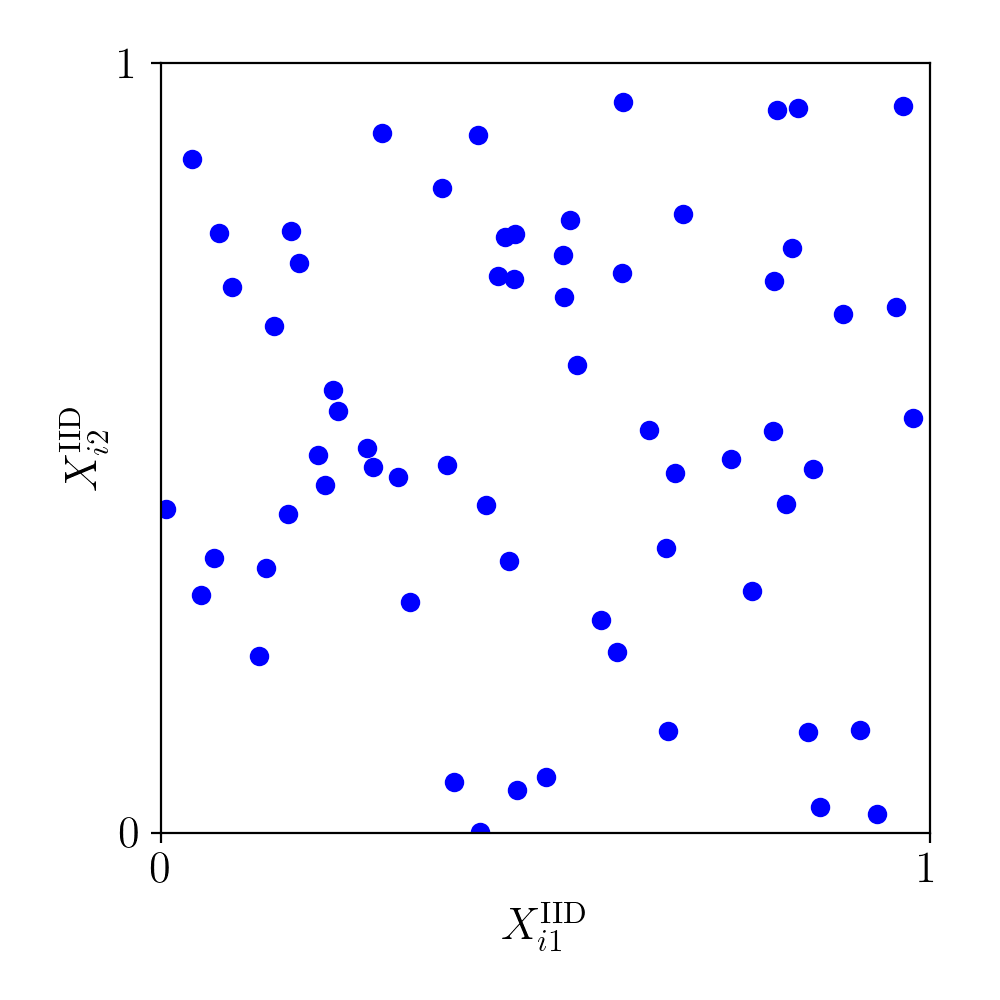
\includegraphics[height=5cm]{ags/figs/dd.iid_uniform_pts.png}%{ProgramsImages/IIDPoints.eps} 
	\qquad
	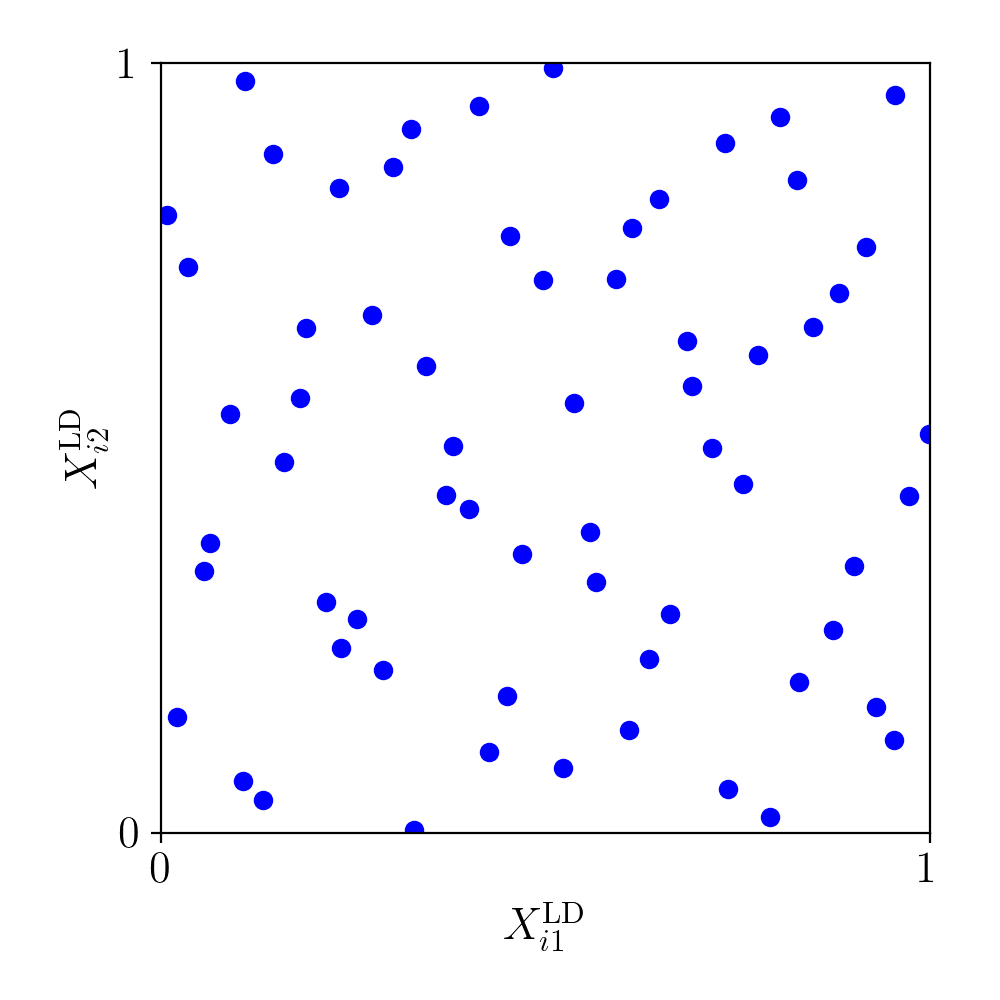
\includegraphics[height=5cm]{ags/figs/dd.sobol_pts.png}%{ProgramsImages/SSobolPoints.eps}
	\caption{IID points contrasted with LD points.  The LD points cover the square more evenly. \AGSComment{Changed above figs.}} \label{fig:comparePts}
\end{figure}

LD points may be deterministic or random, but each point is carefully coordinated with the other so that they fill the square well.  When we say that $\bsX_0, \bsX_1, \ldots \LDsim F$, we mean that for any positive integer $n$,  the empirical distribution of $\bsX_0, \ldots, \bsX_{n-1}$, denoted $F_{\{\bsX_i\}_{i=0}^{n-1}}$,  approximate the target distribution, $F$, well (relative to $n$).  (The empirical distribution of a set assigns equal probability to each point.)  The measure of the difference between the empirical distribution of a set of points and the target distribution is called a \emph{discrepancy} and is denoted $D(\{\bsX_i\}_{i=0}^{n-1}, F)$.  This is the origin of the term low discrepancy points.  LD points by definition have a smaller discrepancy than IID points.  Figure \ref{fig:comparePts} contrasts IID uniform points with LD points, $\bsX^{\LD}_0, \bsX^{\LD}_1 \ldots \LDsim \calU[0,1]^2$, in this case linearly scrambled Sobol' points. For most LD sequences, the target distribution is $\calU[0,1]^d$.

The error of the sample mean in approximating the integral can be bounded according to the Koksma-Hlawka and its extensions as the product of the discrepancy of the sampling sequence and the variation of the integrand, denoted $V(\cdot)$:
\begin{equation}
	\QMCPYabs{\mu - \hmu} = \QMCPYabs{\int_{\calX} f(\bsx) \, \D (F - F_{\{\bsX_i\}_{i=0}^{n-1}}) (\bsx)} \le D(\{\bsX_i\}_{i=0}^{n-1}, F) V(f),
\end{equation} 
The variation is a (semi-) norm of the integrand in a suitable Banach space.  The discrepancy corresponds to the norm of the error functional for that Banach space.  For typical Banach spaces, the discrepancy of LD points is $\calO(n^{-1+\epsilon})$, which is a higher convergence order than for IID points.  For details, the reader is referred to the references.  For our purposes, we hope  that the reader sees here in Figure \ref{fig:comparePts} that the LD points cover the integration domain more evenly than IID points and that in the examples below the reader will see the demonstrably smaller cubature errors.

In the sections that follow we first overview available QMC software.  We next describe an architecture for good QMC software, i.e., what are the key components and how should they interact.  We then describe how we have implemented this architecture in QMCPy.  Finally, we summarize further directions that we hope QMCPy and related software projects will take.  Those interested in following the development of QMCPy or even contributing to its growth are urged to visit the GitHub repository at \href{https://qmcsoftware.github.io/QMCSoftware/}{\nolinkurl{https://qmcsoftware.github.io/QMCSoftware/}}.

\section{Available Software for QMC} \label{sec:available} 
QMC software spans three categories:  LD sequence generators, algorithms, and applications.  We review the better known software collections, recognizing that some software overlaps multiple categories.
Software focusing on generating high quality LD sequences  or their generators includes
\begin{description}[format=\textup,format=\textbf]
% https://tex.stackexchange.com/questions/74279/how-to-add-bullets-to-description-lists
	\item[BRODA] Sobol' sequences in C, MATLAB, and Excel \cite{BRODA20a},
	\item[Burkhardt] various QMC software in C++, Fortran, MATLAB, \& Python \cite{Bur20a},
	\item[LatNet Builder] Generating vectors/matrices for lattices and digital nets \cite{LatNet},
	\item[MATLAB] Sobol' and Halton sequences, commercial \cite{MAT9.9},
	\item[MPS] Magic Point Shop, lattices and Sobol' sequences \cite{Nuy17a},
	\item[Owen] Randomized Halton sequences in R \cite{Owe20a},
	\item[PyTorch] Scrambled Sobol' sequences \cite{PyTorch},
	\item[QMC.jl] LD Sequences in Julia \cite{Rob20a}, and
	\item [qrng]  Sobol' and Halton sequences in R \cite{QRNG2020}.
\end{description}
Software focusing on QMC algorithms and applications includes
\begin{description}[format=\textup,format=\textbf]
	\item[GAIL] Automatic (Q)MC stopping criteria in MATLAB \cite{ChoEtal20a},
	\item[ML(Q)MC] Multi-Level (Quasi-)Monte Carlo routines in C++, MATLAB, Python, and R \cite{GilesSoft},
	\item[OpenTURNS] Open source initiative for the Treatment of Uncertainties, Risks 'N Statistics in Python \cite{OpenTURNS},
	\item[QMC4PDE] QMC for elliptic PDEs with random diffusion coefficients \cite{KuoNuy16a},
	\item[SSJ] Stochastic Simulation in Java \cite{SSJ}, and
	\item[UQLab] Framework for Uncertainty Quantification in MATLAB \cite{UQLab2014}.
\end{description}

The sections that follow describe QMCPy \cite{QMCPy2020a}, which is our attempt to combine the best of the above software under a common user interface written in Python 3.  The choice of language was determined by the desire to make QMC software accessible to a broad audience, especially the tech industry.


\section{Components of QMC Software}
QMC cubature can be summarized as follows.  We want to approximate $\mu$ well by $\hmu$, where \eqref{eq:integral}, \eqref{eq:fintegral}, and \eqref{eq:samplemean} combine to give
\begin{multline} \label{eq:cubSummary}
	\mu : = \int_\calT g(\bst) \, \lambda(\bst) \, \D \bst  = \bbE[f(\bsX)] = \int_\calX f(\bsx) \, \varrho(\bsx) \, \D \bsx \approx \frac 1n \sum_{i=0}^{n-1} f(\bsX_i) =: \hmu, \\
	 \bsX_0, \bsX_1, \ldots \sim F.
\end{multline}
This required four components, which we implement in QMCPy as abstract classes that can be fleshed out into concrete implementations.

\begin{description}[format=\textup,format=\textbf]
	
	\item[Discrete Distribution] that produces $\bsX_0, \bsX_1, \dots$ mimicking the distribution $F$, which typically is $\calU[0,1]^d$;
	
	\item[True Measure] $\bst \mapsto \lambda (\bst) \D \bst$ that defines the original integral, e.g., Gaussian or Lebesgue;
	
	\item[Integrand] $g$ that  defines the original integral, plus the transformed version, $f$, to fit the discrete distribution; and
	
	\item[Stopping Criterion] that determines how large $n$ should be to ensure that $\QMCPYabs{\mu - \hmu_n} \le \varepsilon$.
\end{description}

The software libraries referenced in Section \ref{sec:available} provide one or more of these components.  QMCPy combines multiple examples of them all.


\section{Discrete Distributions}

LD sequences typically mimic $\calU[0,1]^d$, which we assume here.  Good sequences for other distributions are obtained by transformations in the next section.  

QMCPy implements \emph{extensible} LD sequences, i.e., those that allow practitioners to obtain and use additional $f(\bsX_i)$ without discarding the existing $f(\bsX_i)$.  Halton sequences do not have preferred sample sizes $n$, but integration lattices and digital sequences do.  These latter two also have an elegant group structure, which we summarize here.  

For simplicity we restrict ourselves to the case where the first $2^m$ points of these LD sequences form a group under the addition operator $\oplus$.

\begin{table}
	\centering
	\caption{Properties of lattices and digital net sequences.  Note that they share group properties but also have distinctives.} \label{tab:GroupProp}
\[
	\renewcommand{\arraystretch}{1.3}
\begin{array}{c@{\qquad}c}
	\toprule
	\multicolumn{2}{c}{\text{Define \ldots}} \\
	\multicolumn{2}{c}{\bsZ_1, \bsZ_2, \bsZ_4, \ldots \in [0,1)^d \text{chosen well} } \\
	\multicolumn{2}{c}{
	\bsZ_{i} := i_0  \bsZ_1 \oplus i_1 \bsZ_{2} + i_2  \bsZ_{4} +  i_3  \bsZ_{8} + \cdots 
	\qquad
	\text{for }i = i_0 +i_1 2 + i_2 4 + i_3 8 + \cdots} \\
    \multicolumn{2}{c}{\bsX_i := \bsZ_i \oplus \bsDelta, \qquad \text{where }\bsDelta \IIDsim [0,1)^d} \\  \hline
	\text{Rank-1 Integration Lattices} & \text{Digital Nets} \\
		\bst \oplus \bsx : = (\bst + \bsx) \bmod \bsone & \bst \oplus \bsx := \text{binary digitwise addition} \\ 
		 \text{require } \begin{array}{l} \bsZ_1 = (1/2, \ldots, 1/2) \\
		 	\bsZ_{2^{m}} \oplus \bsZ_{2^{m}} = \bsZ_{2^{m-1}} \quad \forall m \in \bbN \end{array}
		\\
\toprule
\multicolumn{2}{c}{\text{Then it follows that \ldots}} \\
	\multicolumn{2}{c}{\begin{array}{r}
			\calP_m := \{\bsZ_0, \ldots, \bsZ_{2^m-1}\}, \quad
			\bsZ_i \oplus \bsZ_j \in \calP_m \\
			\calP_{\bsDelta,m} := \{\bsX_0, \ldots, \bsX_{2^m-1}\}, \quad
			\bsX_i \oplus \bsX_j \ominus \bsX_k \in \calP_{\bsDelta,m}
	\end{array} \quad \begin{array}{l}\forall  i,j,k \in \{0, \ldots, 2^{m} -1\} \\ \forall m \in \bbN_0\end{array}}
\end{array}
\]
\end{table}

We illustrate the difference between lattice and Sobol' sequences using QMCPy.  After installing and importing QMCPy via the Python commands
\lstinputlisting[style=Python]{ags/python/qmcpy_install.py}
we create an instance of a $d=2$ dimensional instance of a \texttt{Lattice} object of the  \texttt{DiscreteDistribution} abstract class.  Then we generate the first eight (non-randomized) points in this lattice:
\lstinputlisting[style=Python]{ags/python/first_Lattice.py}
\FJHComment{Can we set the listlistings style to break long lines of code?}
The first three generators for this lattice are $\bsZ_1 = (0.5, 0.5)$, $\bsZ_2 = (0.25, 0.75)$, and $\bsZ_4 = (0.125, 0.875)$.  One can check that $(\bsZ_2 + \bsZ_4) \bmod \bsone = (0.375, 0.625) = \bsZ_6$, as Table \ref{tab:GroupProp} specifies.

The randomized shift has been turned off above to illuminate the group structure.  In practice, we normally include the randomization to ensure that there are no points on the boundary of $[0,1]^d$.  Then, when points are transformed to mimic distributions with such as the Gaussian, no LD points will be transformed to infinity.

Now, we generate Sobol' points using a similar process as we did for lattice points.  Sobol' sequences are one of the most popular example of digital sequences.
\lstinputlisting[style=Python]{ags/python/first_Sobol.py}
Here, $\bsZ_4$ differs from that for lattices, but more importantly, the definition of addition for digital sequences is different than that for lattices.  Using digitwise addition for digital sequences, we can confirm that according to Table \ref{tab:GroupProp},
\[
\bsZ_2 \oplus_{\dig} \bsZ_4 = ({}_20.010,{}_20.110)  \oplus_{\dig} ({}_20.001,{}_20.101) = ({}_20.011,{}_20.011) = \bsZ_6.
\]

By contrast, if we construct a digital sequence using the generators for the lattice above, we would obtain
\begin{multline*}
\bsZ_6 = (\bsZ_2 + \bsZ_4) \bmod \bsone  = ({}_20.010,{}_20.110)  \oplus_{\dig} ({}_20.001,{}_20.111)  \\
= ({}_20.011,{}_20.0.001) = (0.0375, 0.0375),
\end{multline*}
which differs from the $\bsZ_6$ constructed for lattices.  Thus, lattices and digital sequences are different sets, even if they share the same generators.

The examples of \texttt{gp.Lattice} and \texttt{gp.Sobol} illustrate how QMCPy LD generators share a common user interface, which includes specifying the dimension, when the instance is constructed and specifying the number of points when the \texttt{gen\_samples} method is called.  Following Python practice, parameters can be input without specifying their names if they are input in the prescribed order.  QMCPy also includes Halton sequences and IID sequences.




QMCPy implements numerous discrete distribution classes, both IID and LD. The abstract properties and methods of the abstract discrete distribution class layout requirements for concrete implementations such as the IID standard uniform generator or Sobol' sequence generator. For example, each discrete distribution has a \texttt{gen\_samples} method that allows the user to draw samples from with the instance. Moreover, QMCPy has built each discrete distribution object to be highly customizable and support auxiliary features such as plotting, seeding, and skipping dimensions. 

The following example shows how to utilize QMCPy's \texttt{Sobol} object to generate samples from a digital net. The construction and usage of other discrete distribution objects uses the same syntax with a uniform API. Note that many of the parameters are defaulted during construction but may be explicitly set for customized usage. 

Docs at \cite{QMCPyDocs}

\AGSComment{Import qmcpy as qp}

\lstinputlisting[style=Python]{ags/python/discrete_distrib.py}

\begin{figure}
	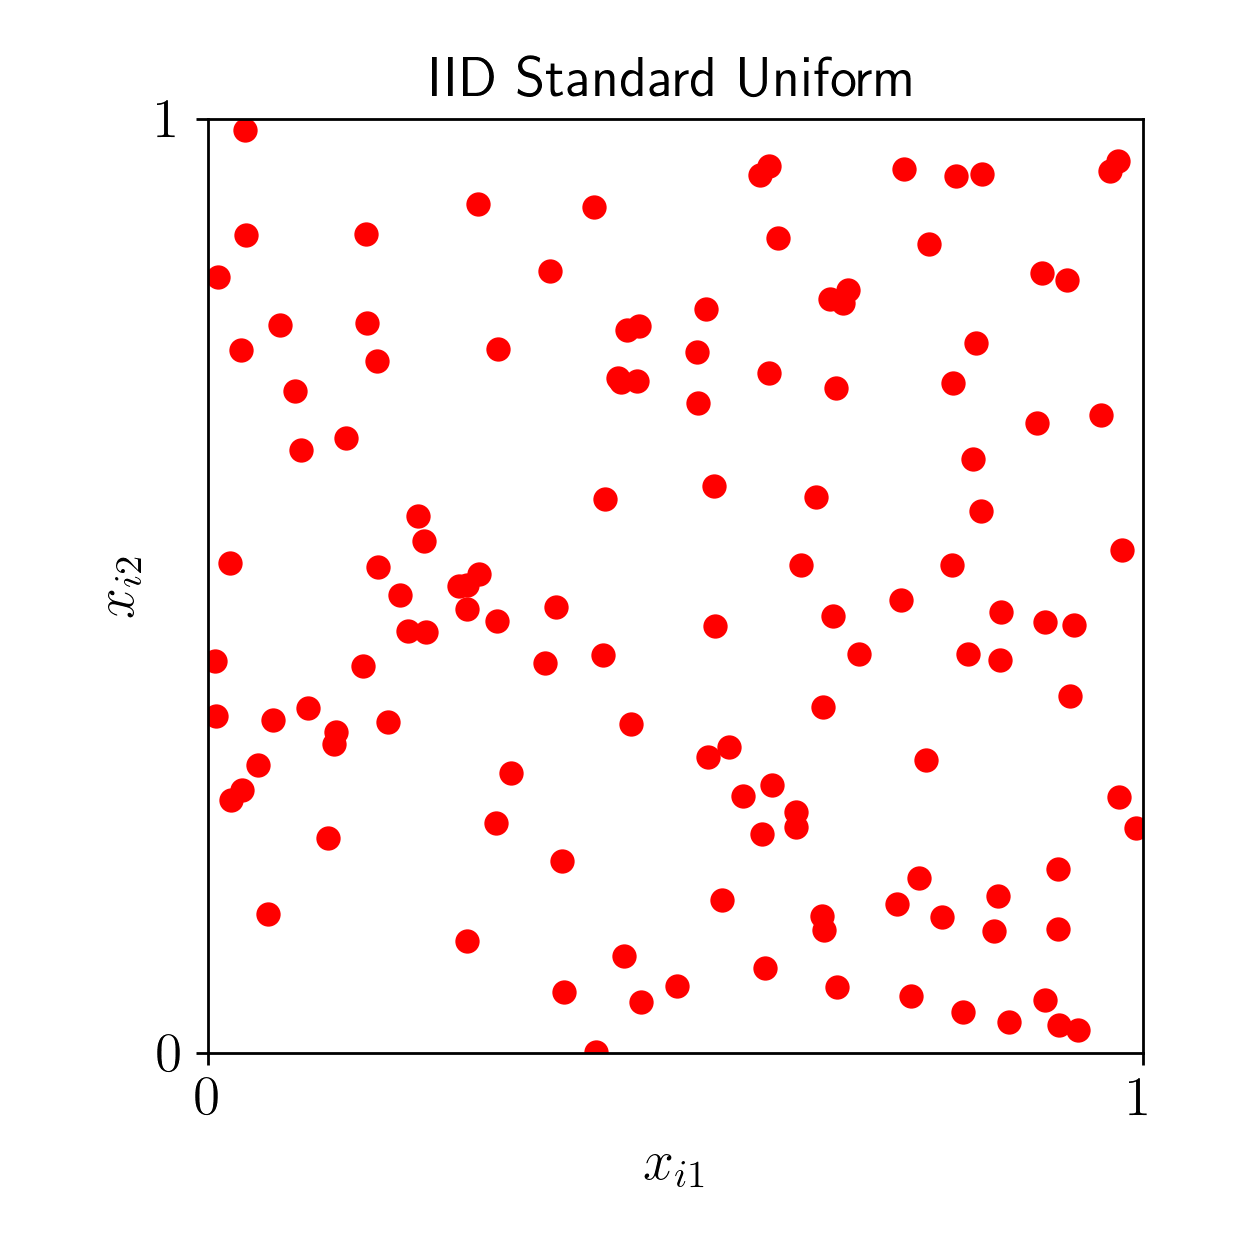
\includegraphics[height=5cm]{ags/figs/dd.iid_std_uniform_1.png}
	\qquad
	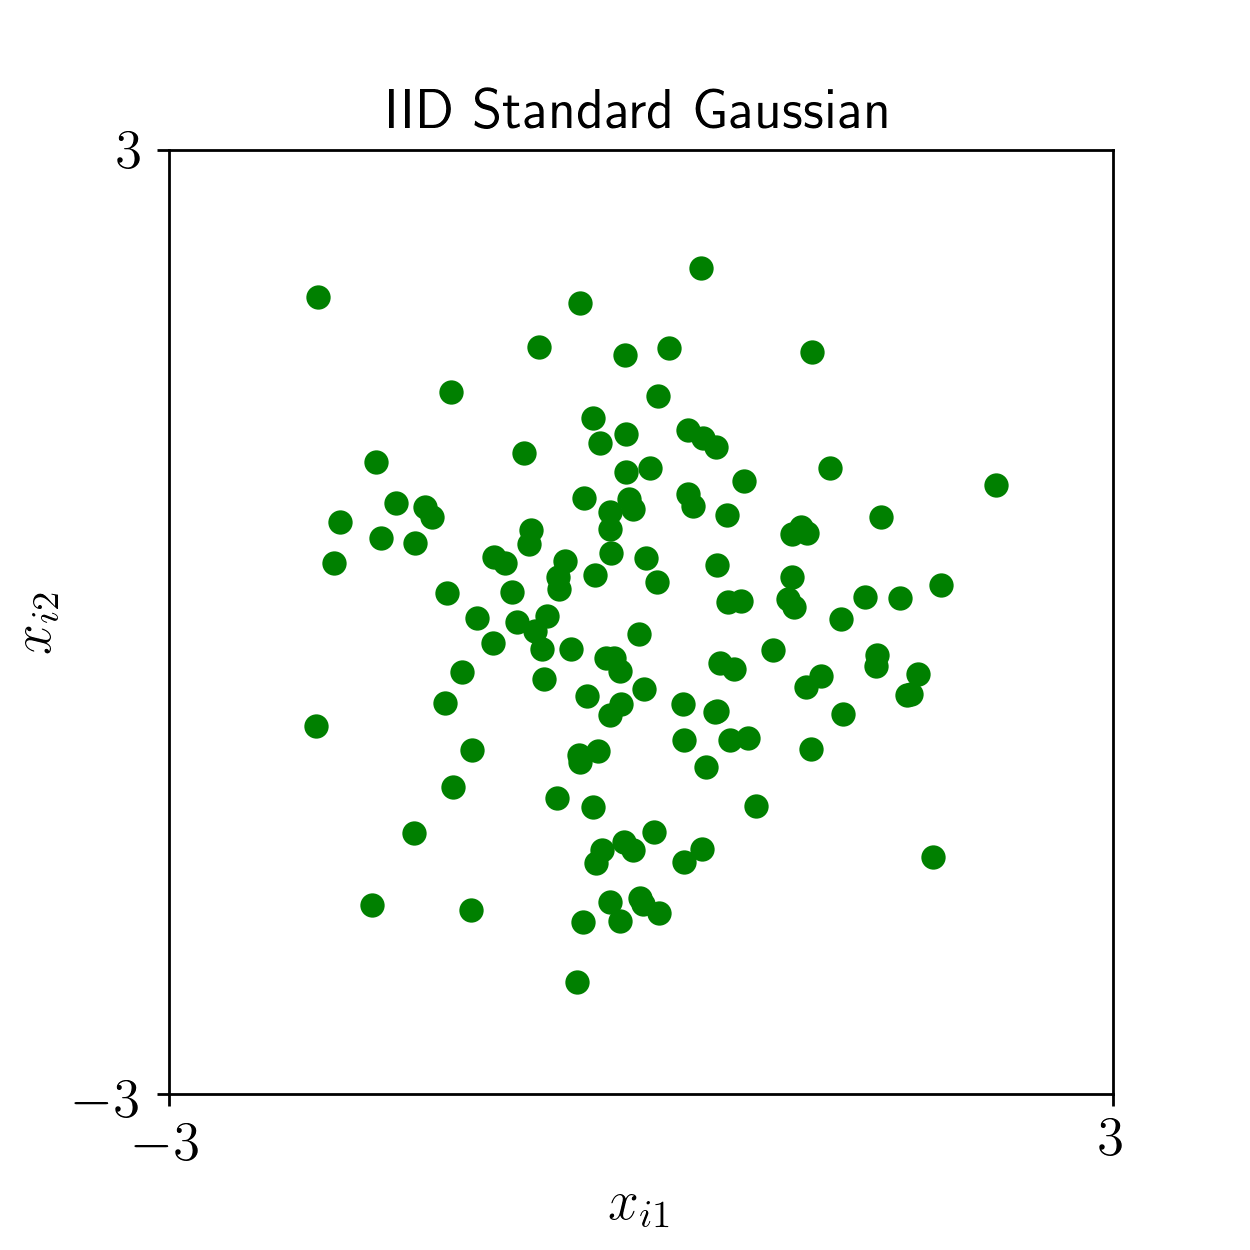
\includegraphics[height=5cm]{ags/figs/dd.iid_std_gaussian.png}
	\caption{\AGSComment{TODO}}
	\label{fig:dd_iid}
\end{figure}

\begin{figure}
	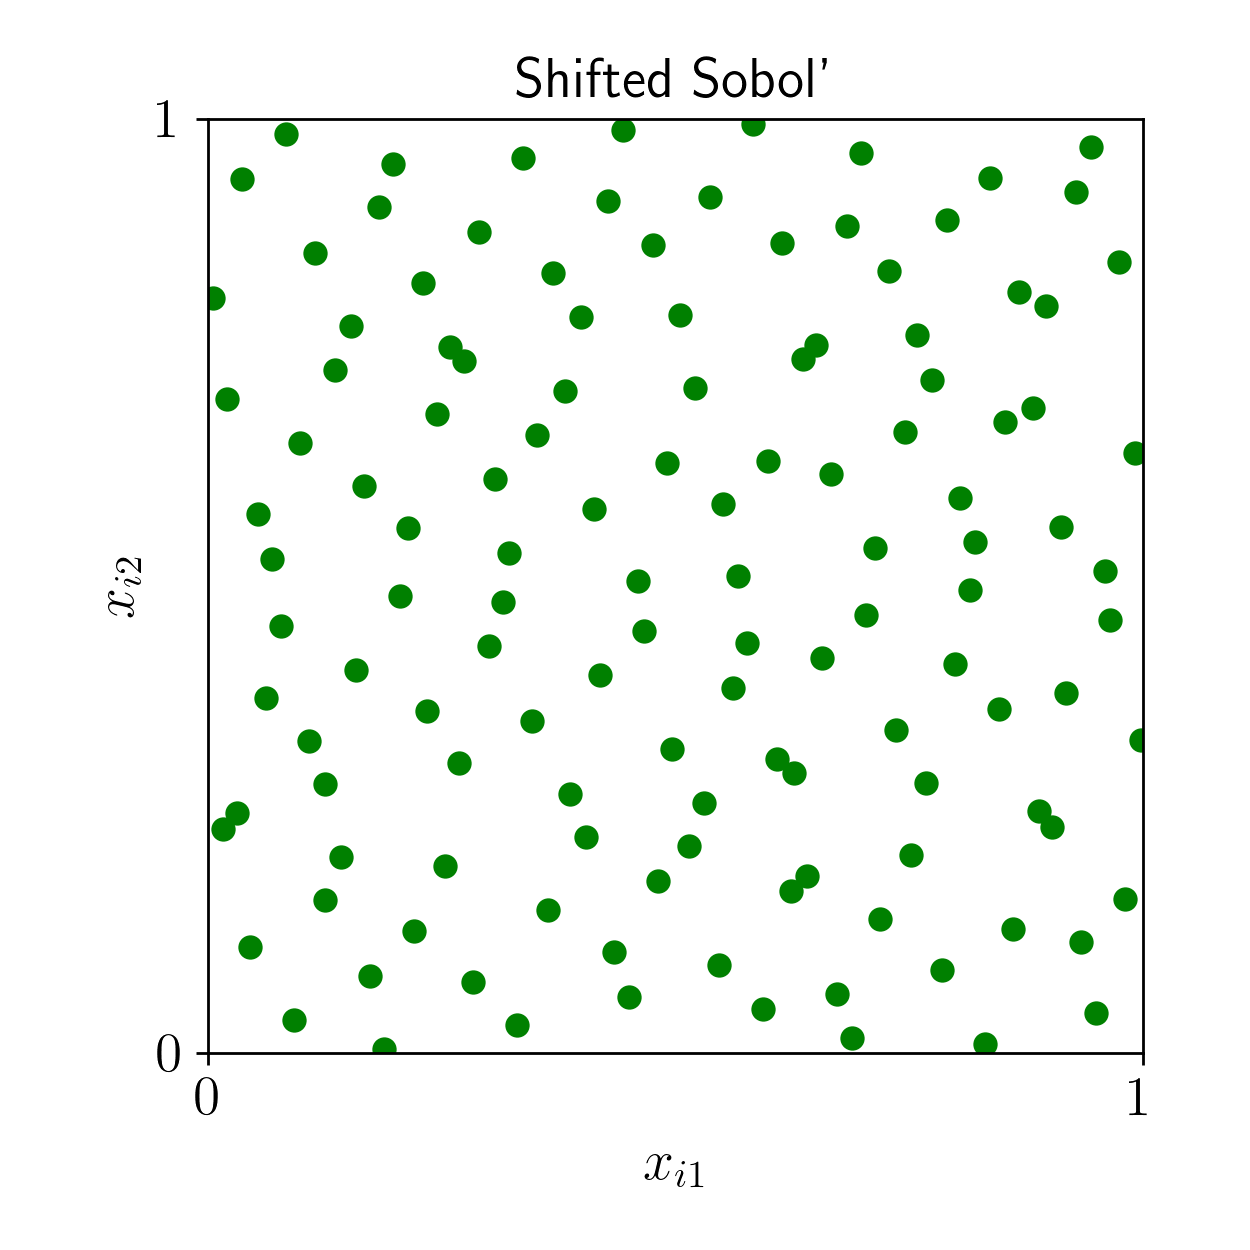
\includegraphics[height=5cm]{ags/figs/dd.sobol.png}
	\qquad
	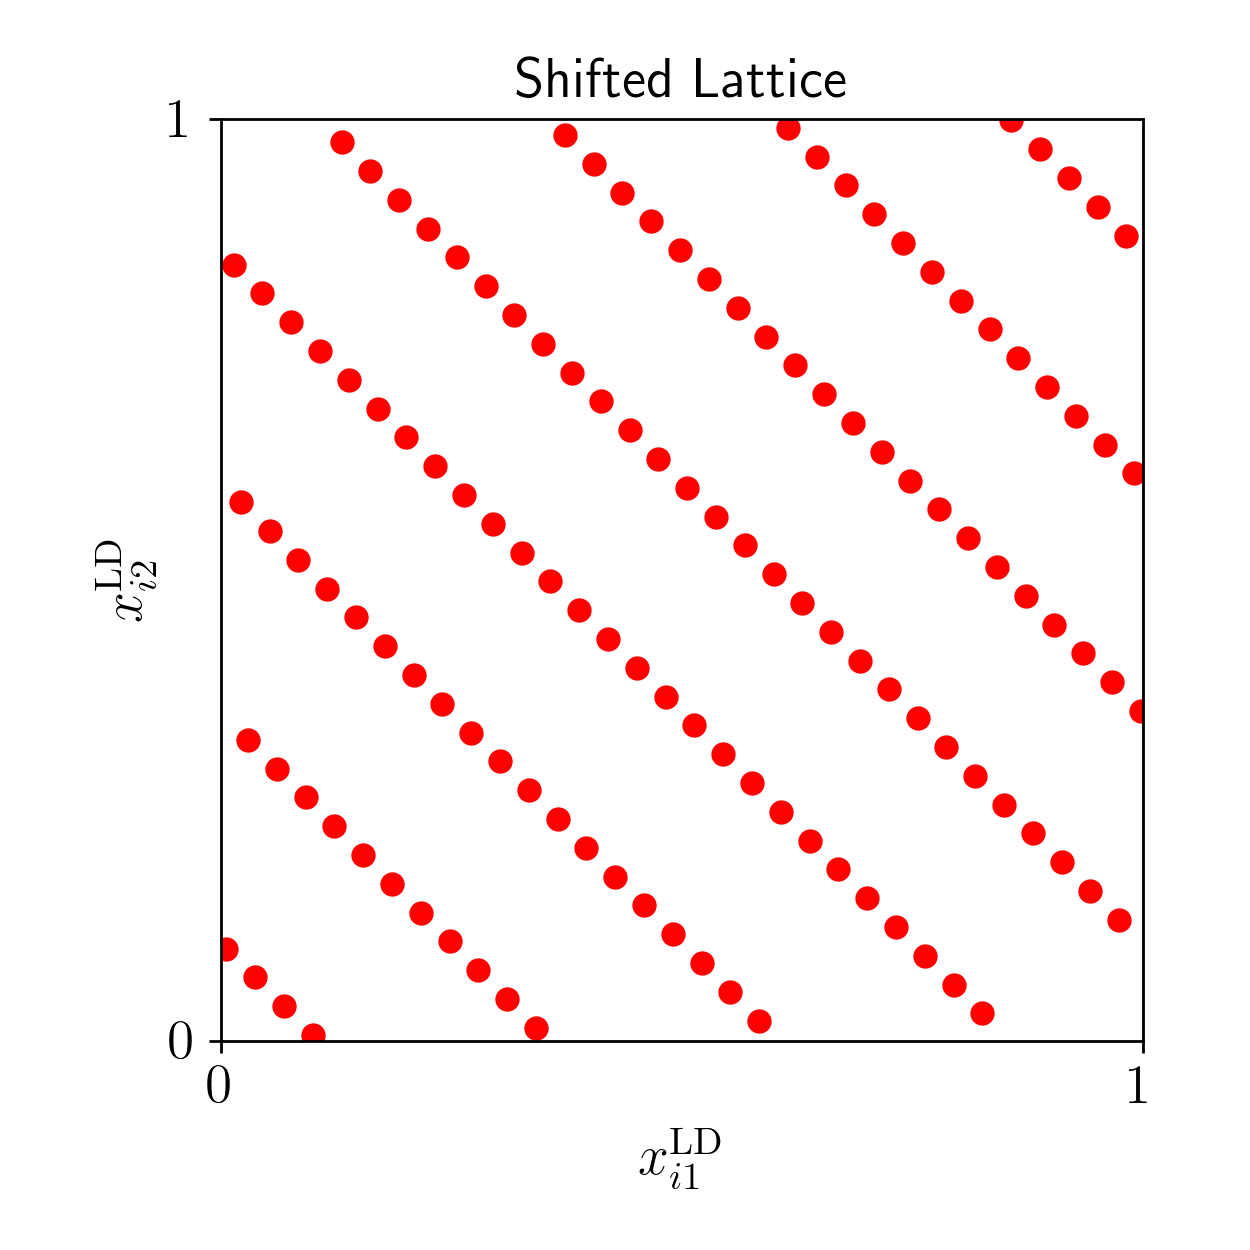
\includegraphics[height=5cm]{ags/figs/dd.lattice.png}
	\qquad
	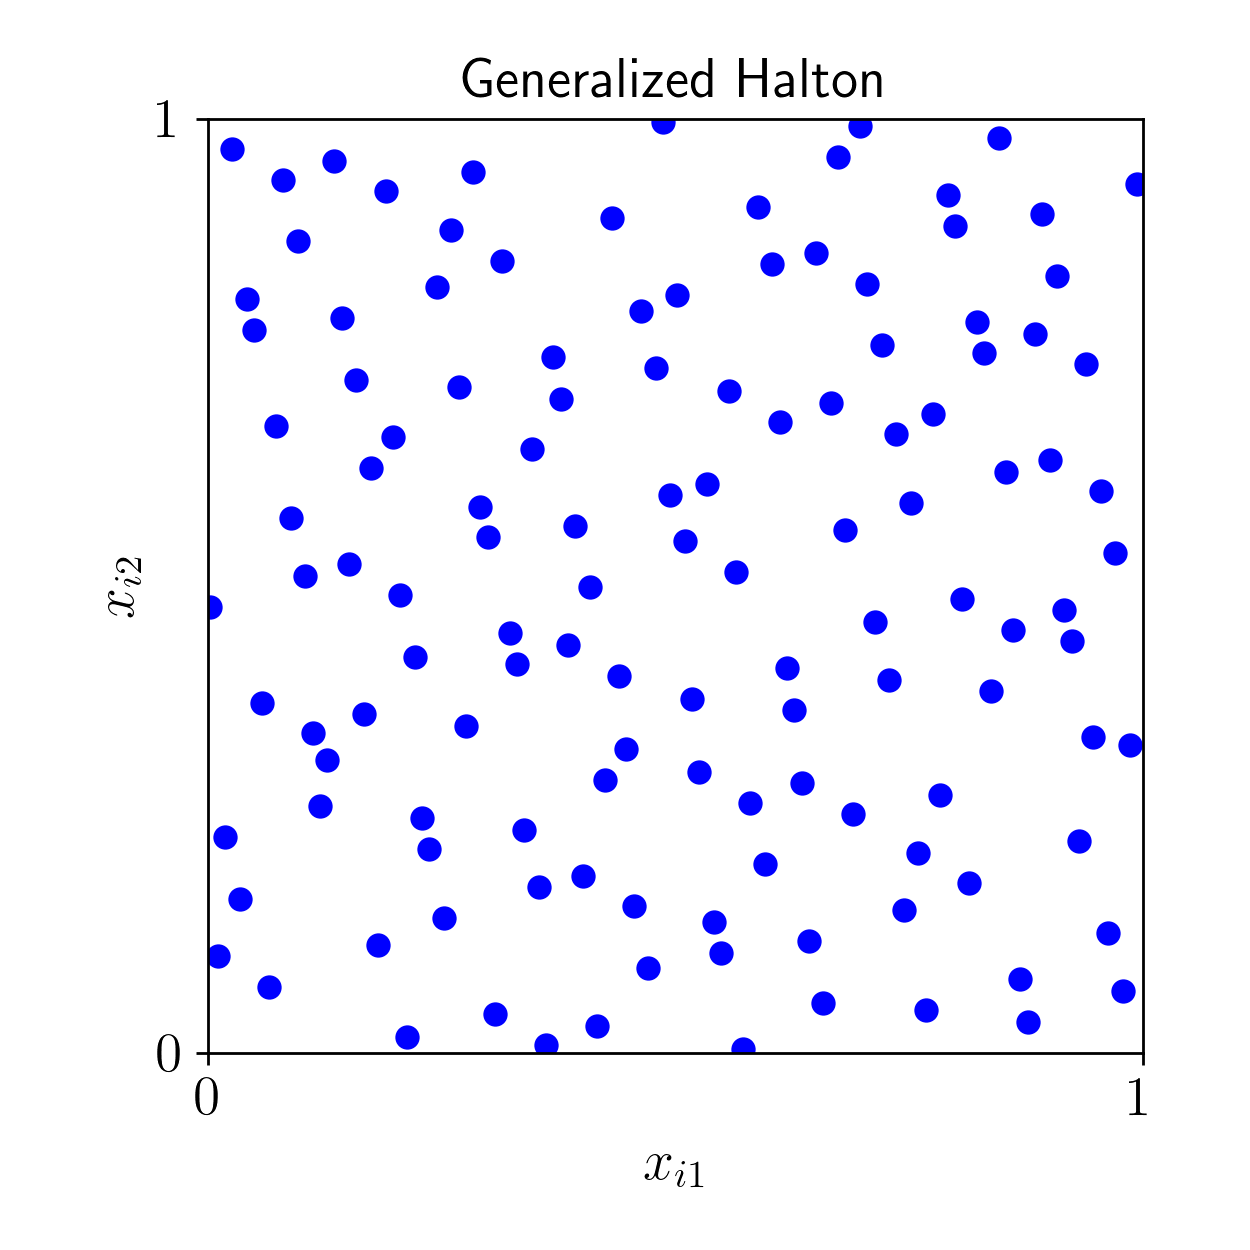
\includegraphics[height=5cm]{ags/figs/dd.halton.png}
	\caption{\AGSComment{TODO}}
	\label{fig:dd_ld}
\end{figure}

\section{True Measure}

\lstinputlisting[style=Python]{ags/python/true_measure.py}

\begin{figure}
	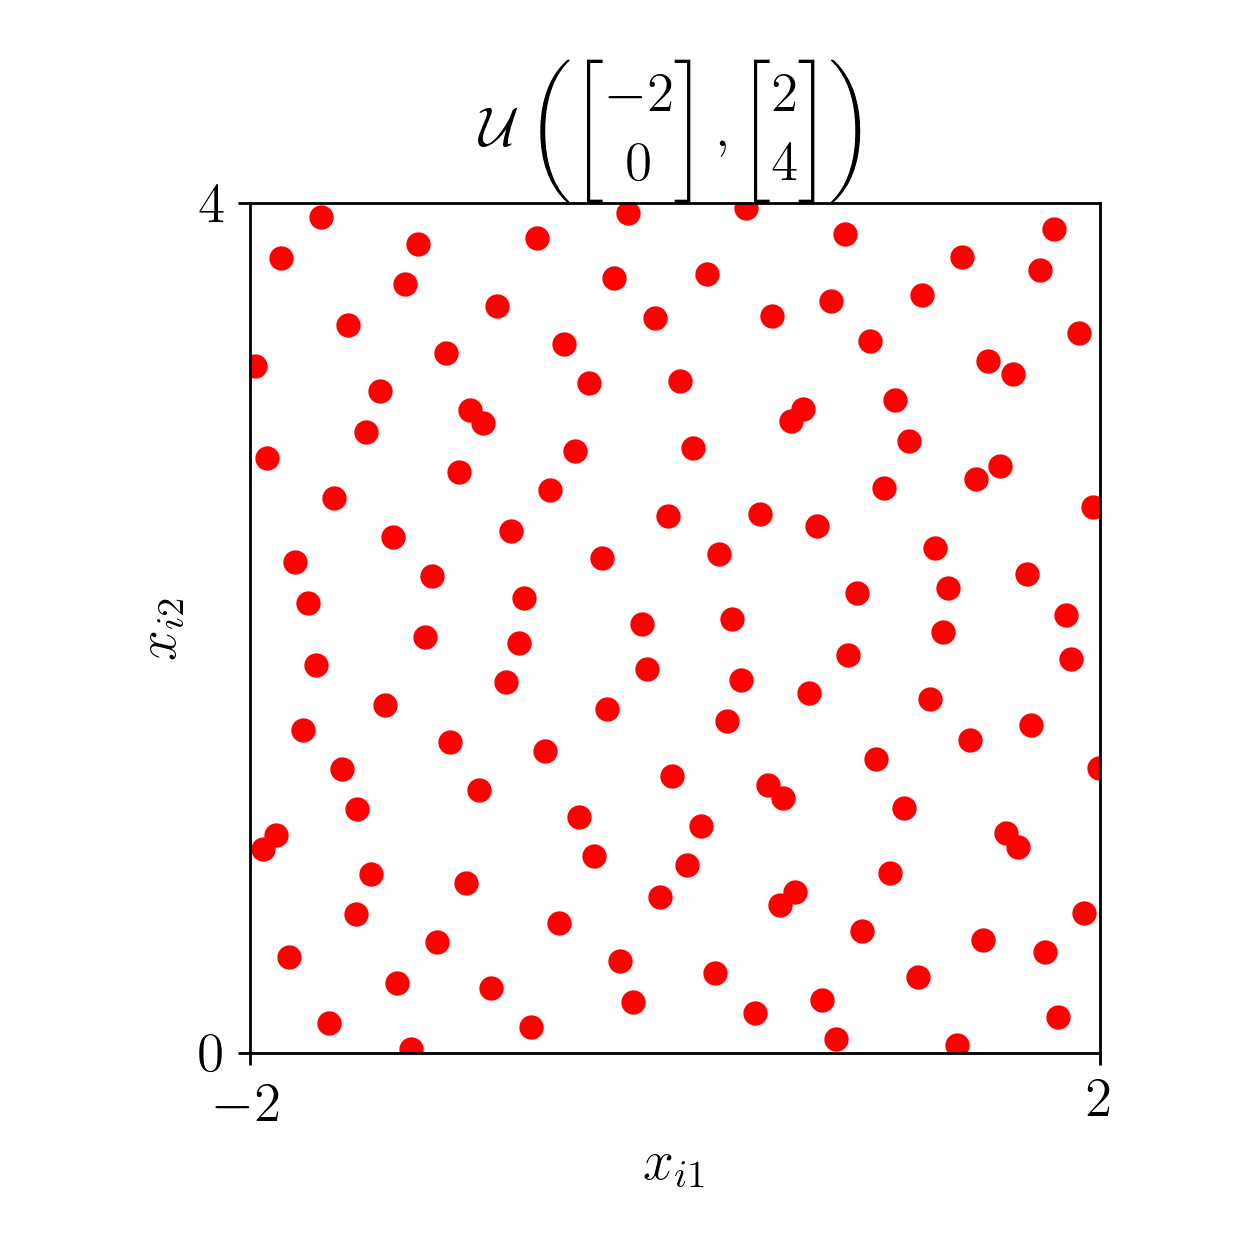
\includegraphics[height=5cm]{ags/figs/tm.uniform.png} 
	\qquad
	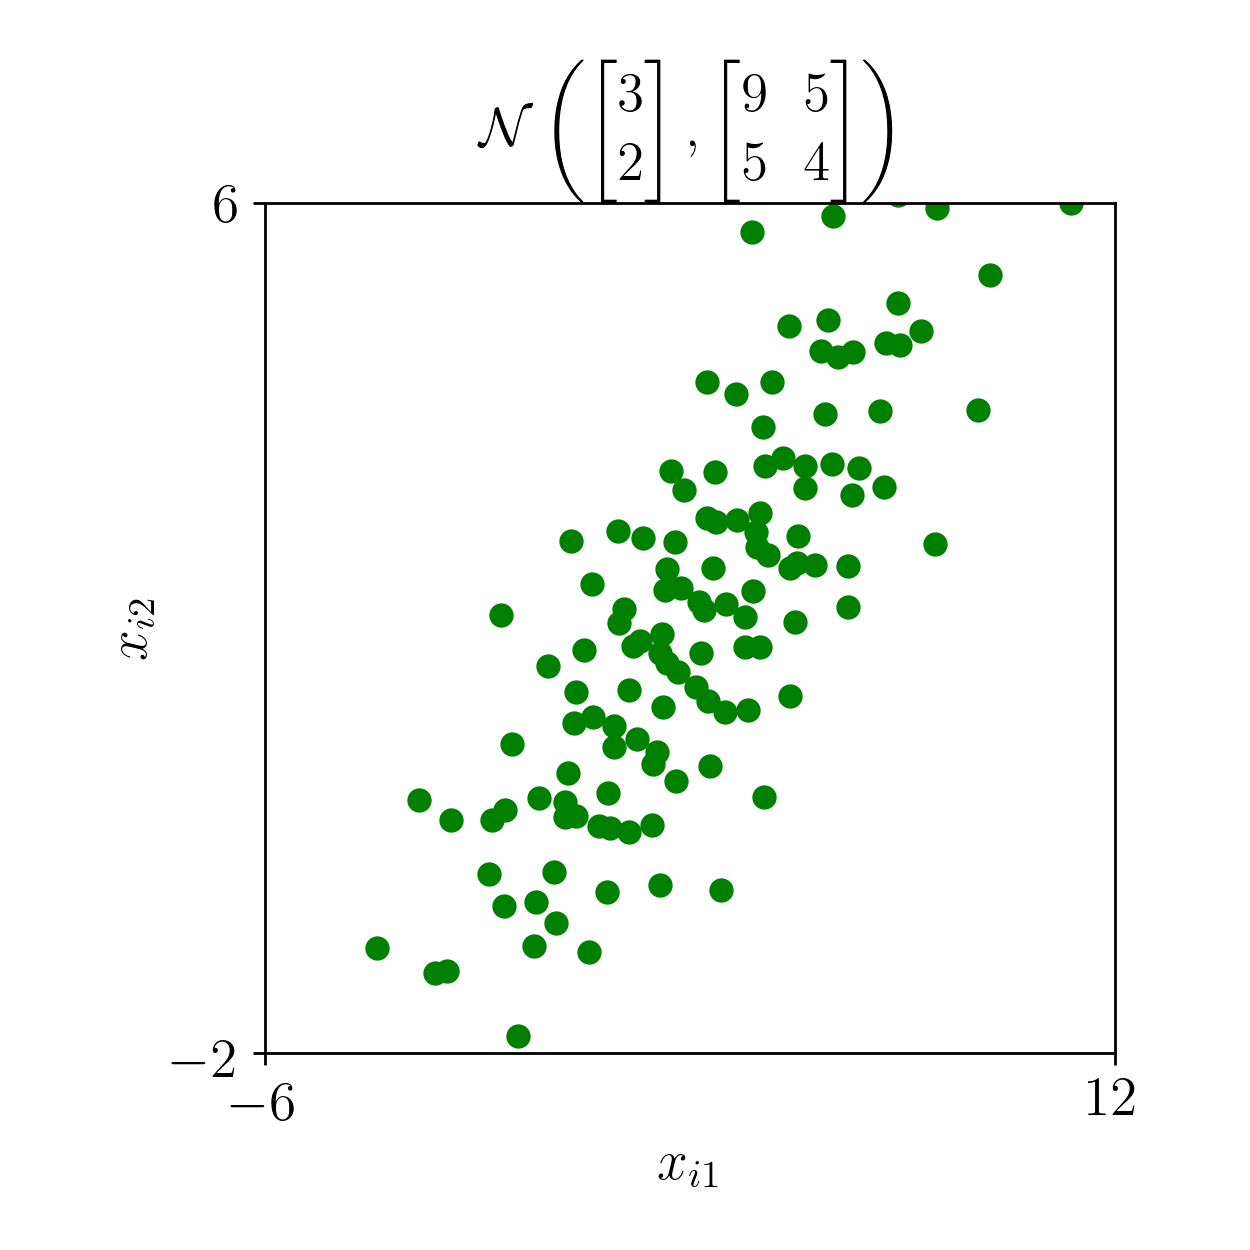
\includegraphics[height=5cm]{ags/figs/tm.gaussian.png}
	\qquad
	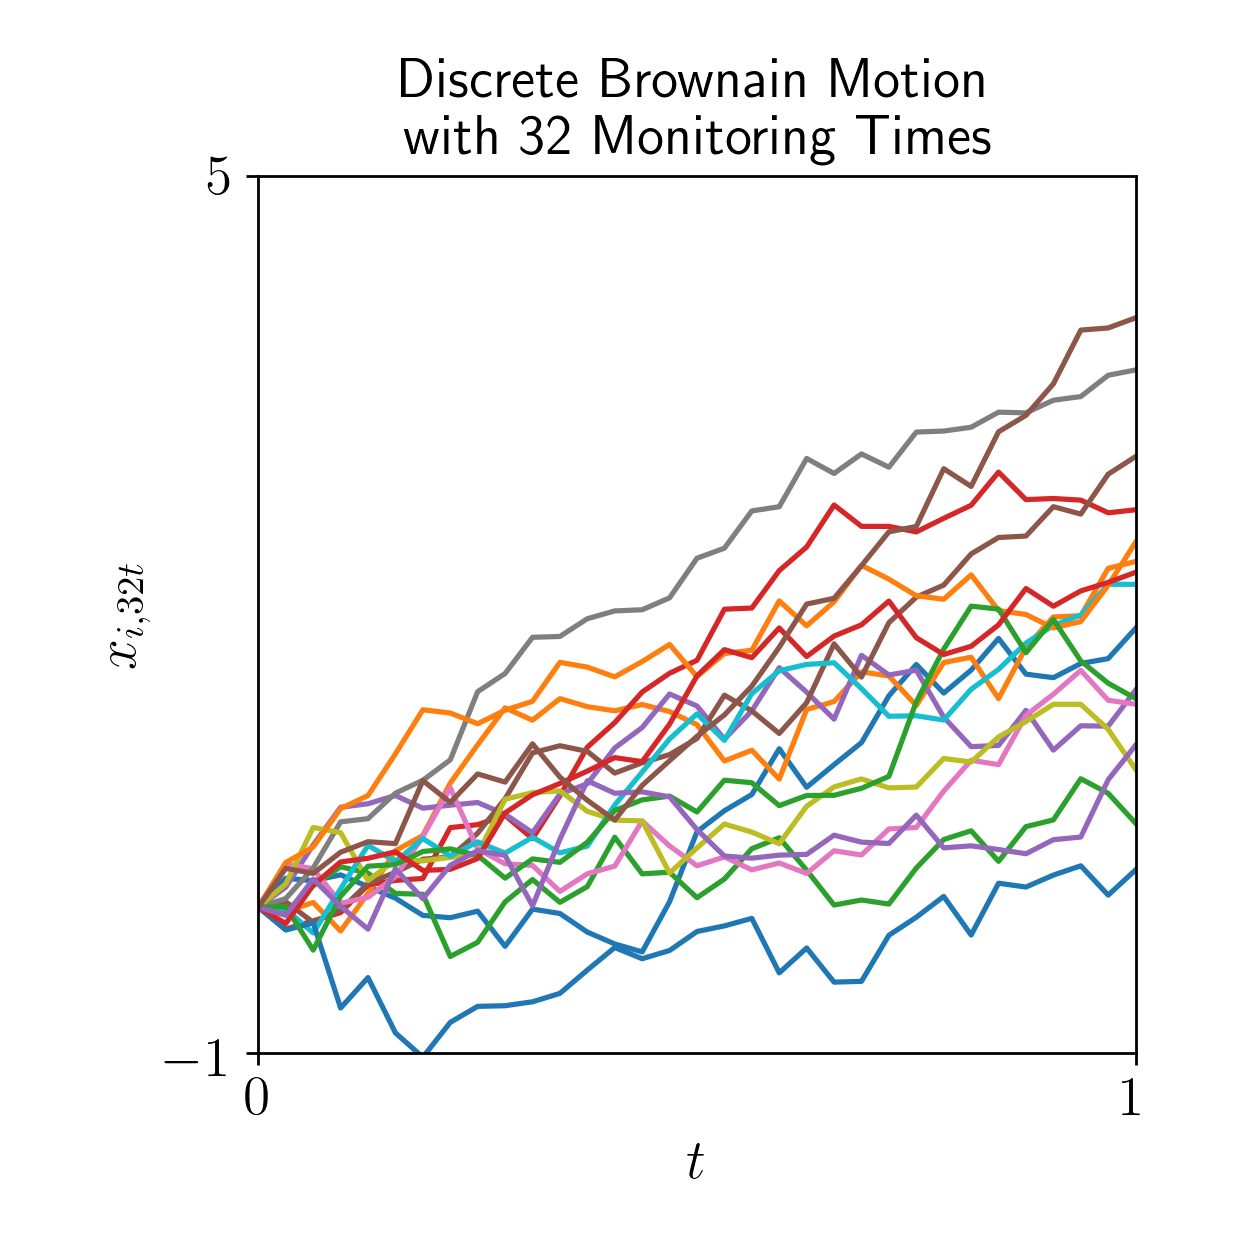
\includegraphics[height=5cm]{ags/figs/tm.brownian_motion.png}
	\caption{\AGSComment{TODO}}
	\label{fig:tm}
\end{figure}

\section{Integrands}

\lstinputlisting[style=Python]{ags/python/integrand.py}

\begin{figure}
	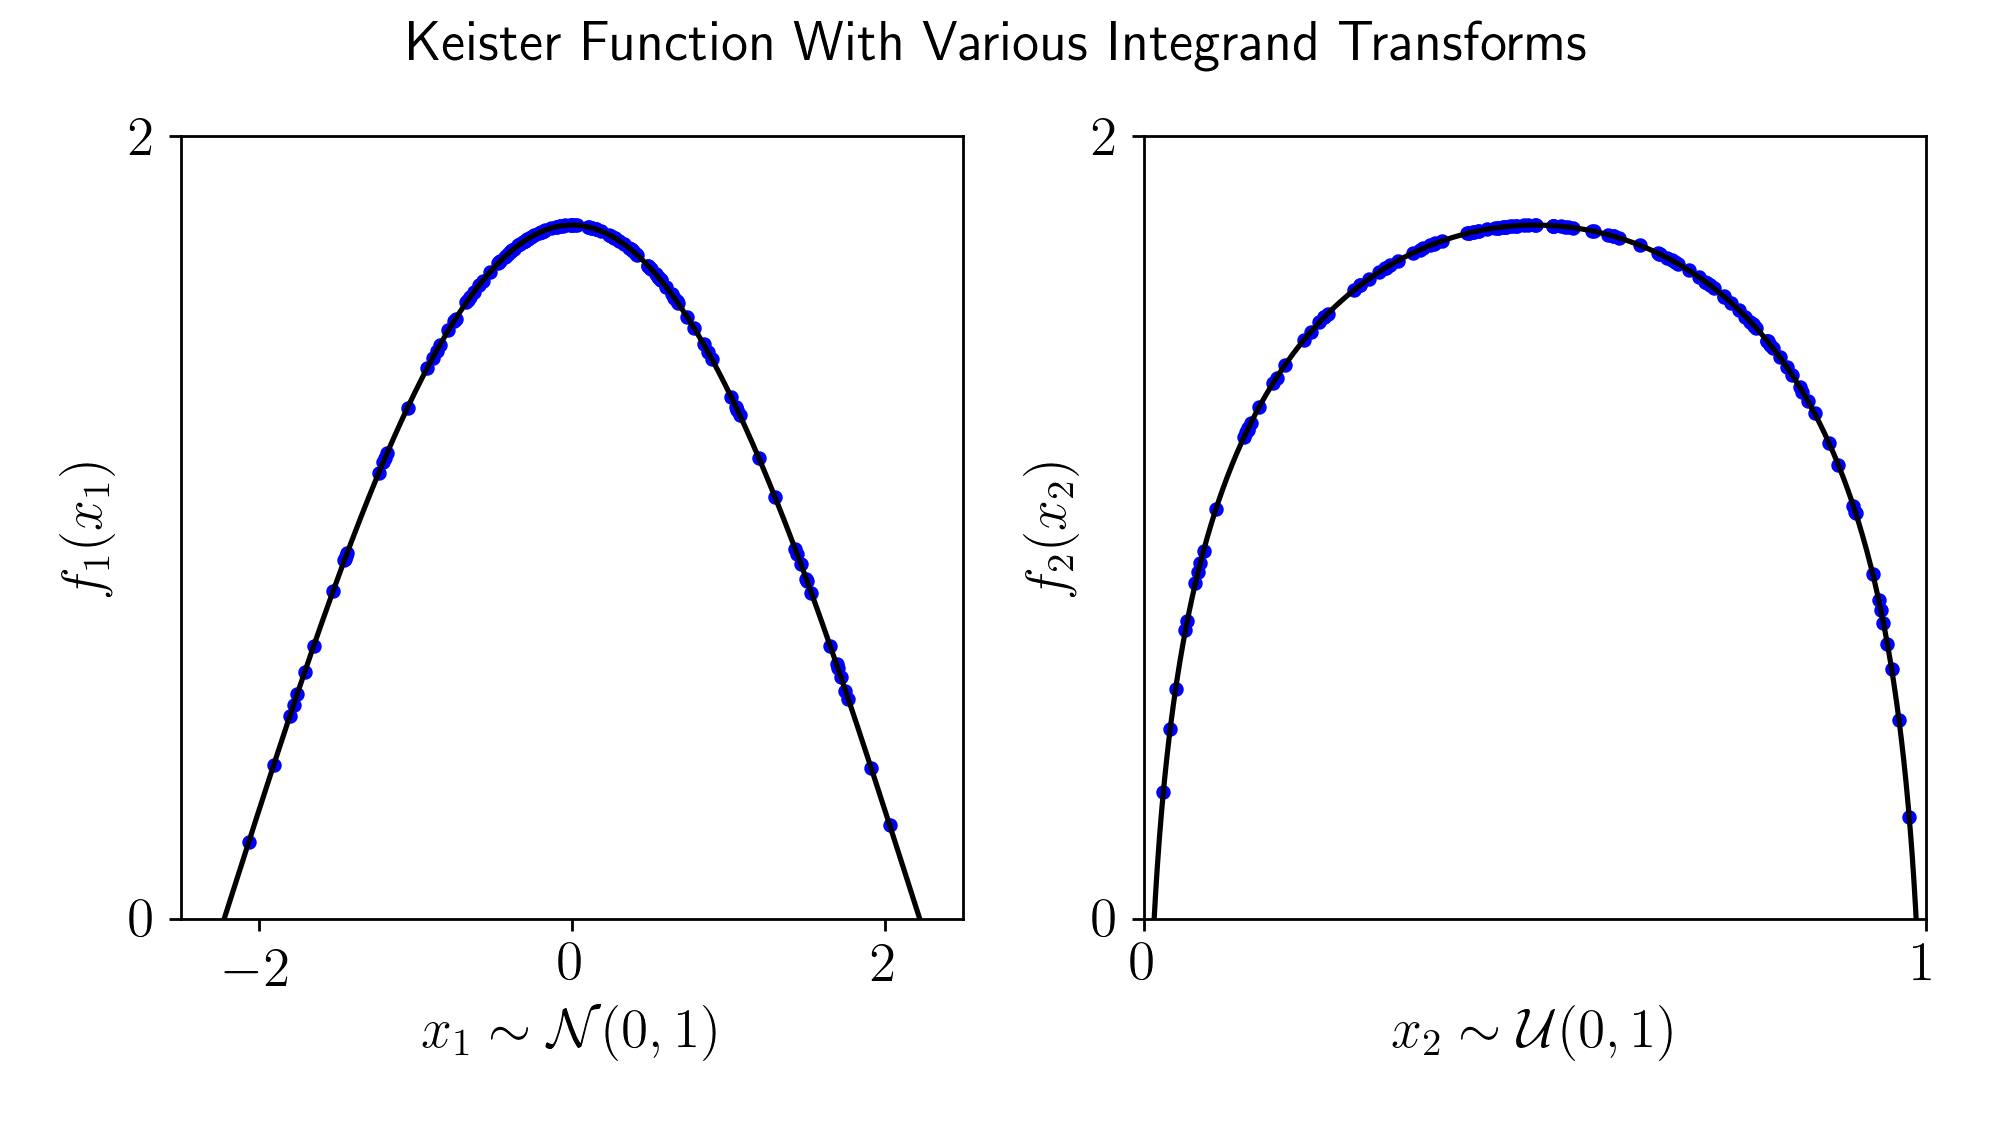
\includegraphics[height=4cm]{ags/figs/i.keister_figs.png}
	\caption{\AGSComment{ToDO}} \label{fig:ikf}
\end{figure}

\begin{figure}
	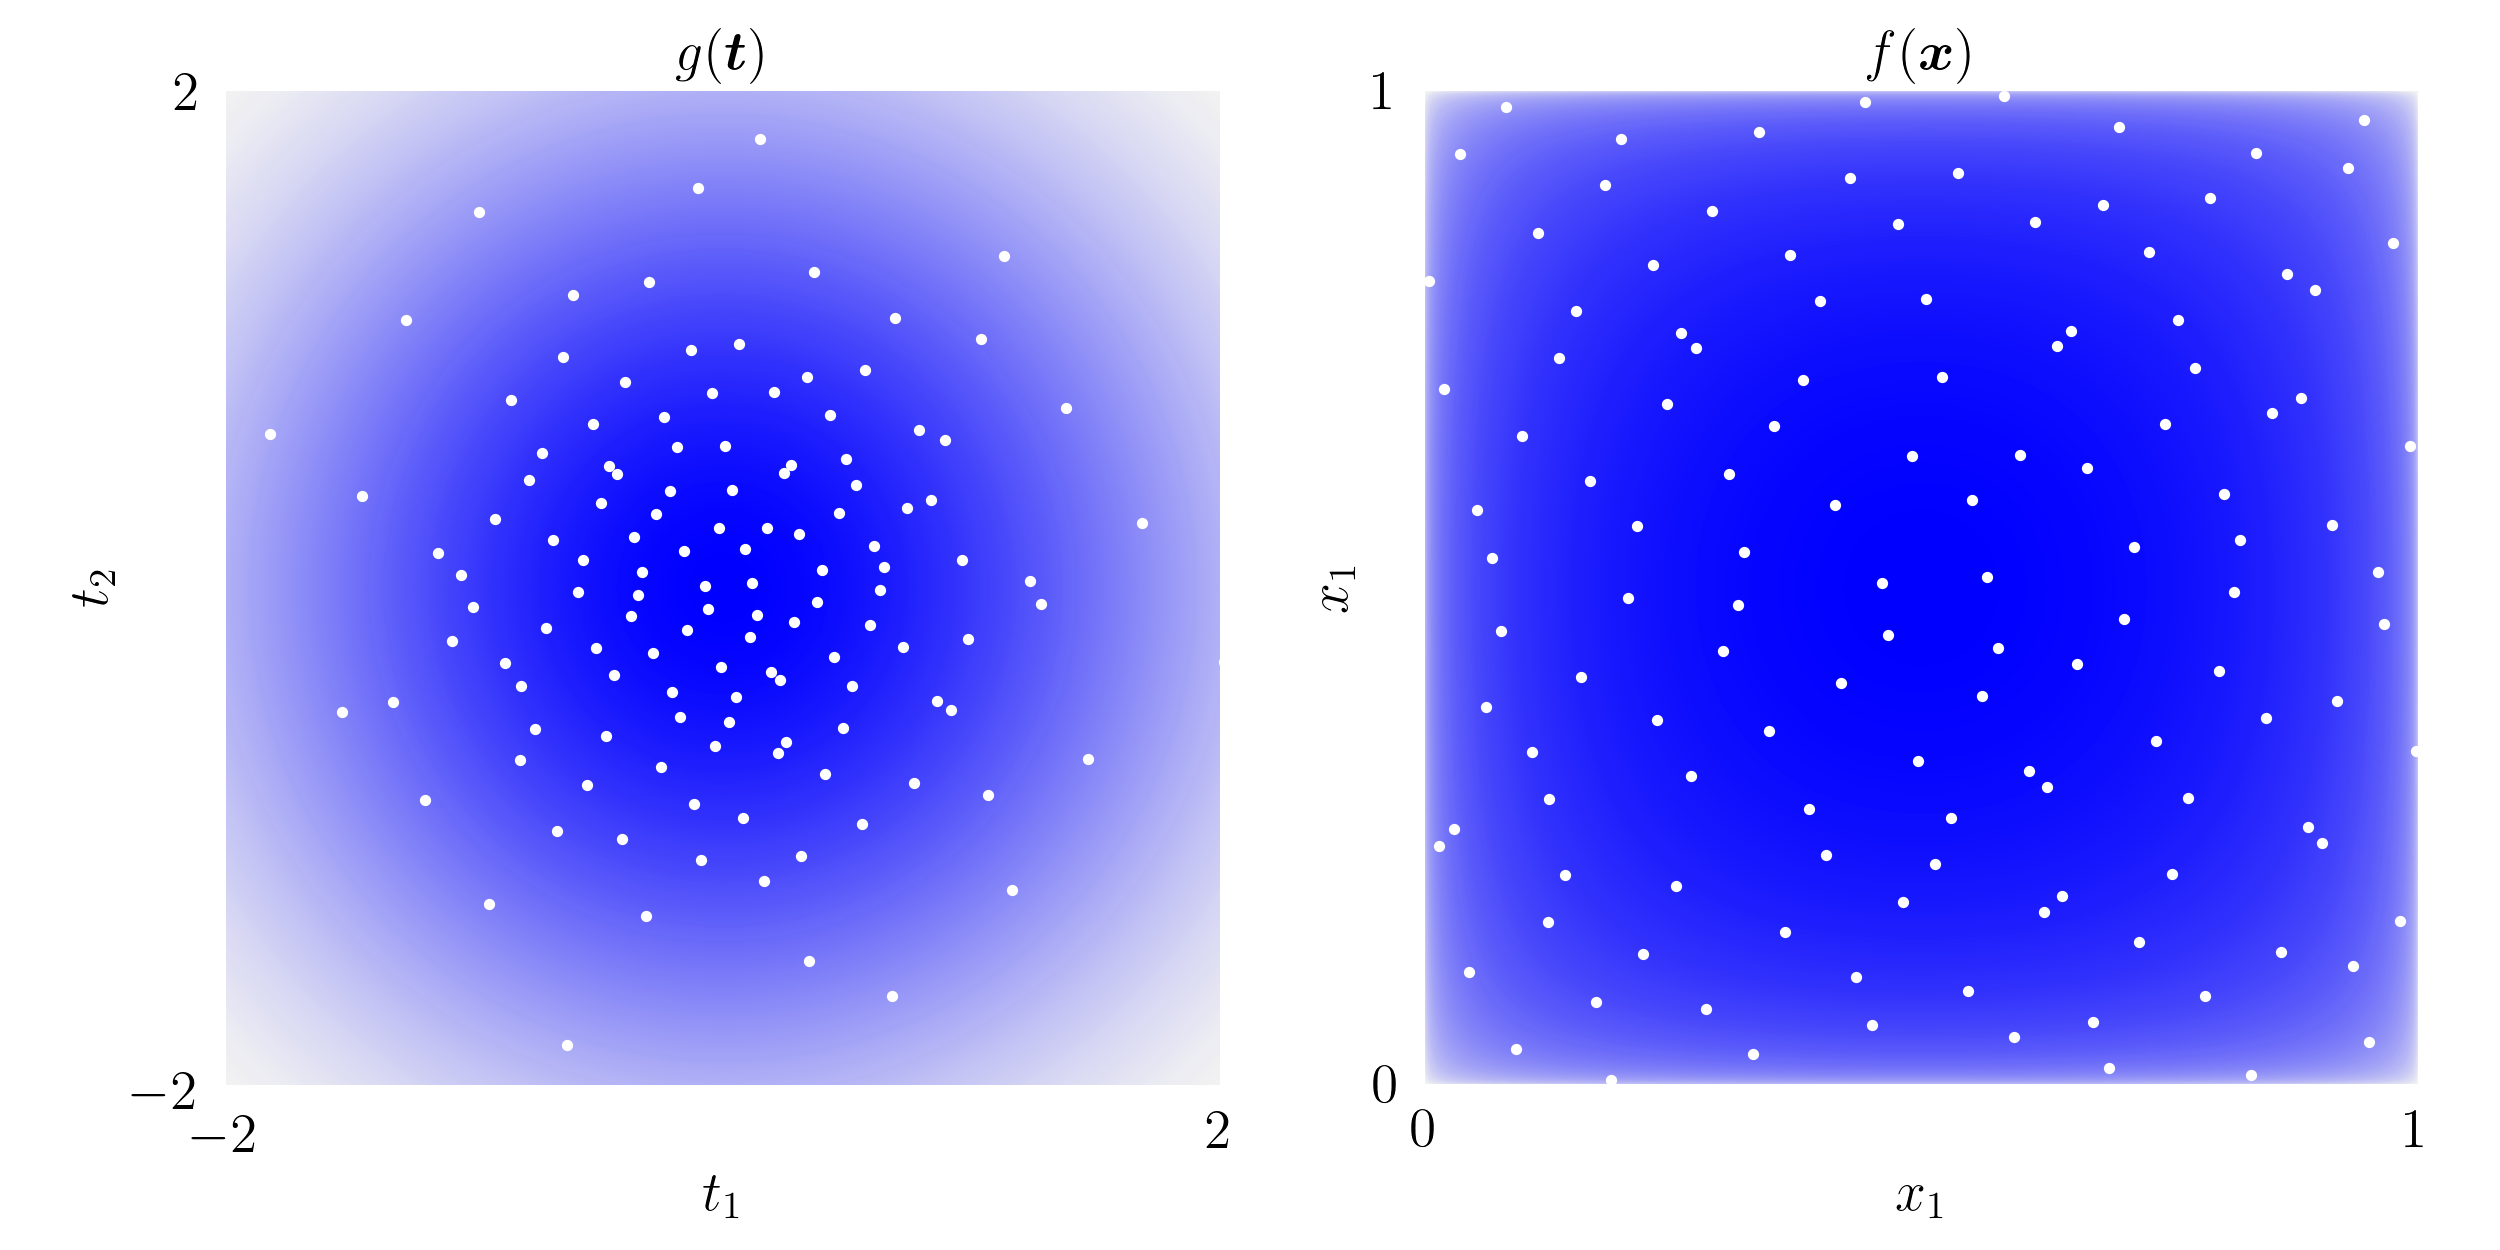
\includegraphics[height=4cm]{ags/figs/i.keister_contours.png}
	\caption{\AGSComment{ToDO}} \label{fig:ikc}
\end{figure}

\section{Stopping Criteria}

\lstinputlisting[style=Python]{ags/python/sc_mc.py}

\lstinputlisting[style=Python]{ags/python/sc_qmc.py}

\section{Under the Hood}

\AGSComment{
\begin{itemize}
    \item \texttt{print} method for all QMCPy objects
    \item custom generating vectors / matrices
    \item \texttt{Sobol} / \texttt{DigitalNet} options unique to QMCPy
    \item \texttt{plot} method for most objects
    \item more option pricing examples? 
\end{itemize}}

\section{Further Work} \label{sec:further}


\begin{acknowledgement}
The authors would like to thank the organizers for a wonderful MCQMC 2020. 
We also thank the referees for their many helpful suggestions.  This work is supported in part by National Science Foundation grants DMS-1522687 and SigOpt.


\end{acknowledgement}

%\section*{References}
%\nocite{*}
\bibliographystyle{spmpsci.bst}
\bibliography{FJH23,FJHown23}


\end{document}

